\documentclass[final,3p,fleqn, 10pt]{elsarticle}
% Recommended, but optional, packages for figures and better typesetting:
\makeatletter
\def\ps@pprintTitle{%
 \let\@oddhead\@empty
 \let\@evenhead\@empty
 \def\@oddfoot{}%
 \let\@evenfoot\@oddfoot}
\makeatother
\usepackage[capposition=top]{floatrow}
\usepackage[utf8]{inputenc}%(only for the pdftex engine)
%\RequirePackage[no-math]{fontspec}%(only for the luatex or the xetex engine)
 \usepackage{url} 
%\usepackage[margin=1in]{geometry} 
\usepackage{setspace}
\usepackage[T1]{fontenc}
\usepackage{lmodern}
\setstretch{1.15}
 
% Packages from D-LATE preamble (potentially useful and not obviously covered by dgruyter)
\usepackage{microtype}
\usepackage{graphicx} % Already used by dgruyter but good to ensure

\usepackage{subfigure} % For subfigures, if any are added later
\usepackage{subcaption} % For subfigure environment
%\usepackage{subcaption}
\usepackage{booktabs} % For professional tables
\usepackage{natbib} % For bibliography management
\usepackage{amsmath} % dgruyter likely includes it, but explicit is safe
\usepackage{amssymb} % dgruyter likely includes it
\usepackage{mathtools} % Extends amsmath
\usepackage{amsthm} % For theorems, dgruyter might have its own, but this is standard
\usepackage{bm} % For \mathbbm{1} (bold math for indicator) - or use dsfont
\usepackage{dsfont} % Alternative for \mathds{1} if \mathbbm{1} is problematic
\usepackage[capitalize,noabbrev]{cleveref} % For smart cross-referencing

% Custom commands and theorem environments from D-LATE preamble
\usepackage{enumitem} % Though lists will be converted to paragraphs
\usepackage{color} % Unlikely needed for final submission

\newcommand{\indep}{\rotatebox[origin=c]{90}{$\models$}}
\newcommand\Norm {\mathcal{N}}
\newcommand\E {\mathbb{E}}
\newcommand\Expect{\E}
% \renewcommand\Re{\R} % \R is already defined below, avoid redefinition conflict if possible
\newcommand\bs {\boldsymbol}
\newcommand\bPsi {\bs{\psi_u}}
% \newcommand\X {\mathcal{X}} % \cX is defined below
\newcommand\bxi {\bs{\xi}}
\newcommand\z {\mathtt z}
\newcommand\Var {\ensuremath{\mathrm{Var}}}
\newcommand\Cov {\ensuremath{\mathrm{Cov}}}
\newcommand\sign {\ensuremath{\operatorname{\mathrm{sign}}}}
\newcommand\sam {\ensuremath{\operatorname{\mathrm{sam}}}}
\newcommand\zu {\mathfrak{z}}
\newcommand*{\defeq}{\stackrel{\textup{def}}{=}}
\newcommand*{\eqdef}{\stackrel{\textup{def}}{=}}
\newcommand\range {\ensuremath{\operatorname{\mathrm{range}}}}
\newcommand\mynull {\ensuremath{\operatorname{\mathrm{null}}}}
\newcommand\rank {\ensuremath{\operatorname{\mathrm{rank}}}}
\newcommand\krank {\ensuremath{\operatorname{\mathrm{krank}}}}
\newcommand\spark {\ensuremath{\operatorname{\mathrm{spark}}}}
\newcommand\conv {\ensuremath{\operatorname{\mathrm{conv}}}}
\newcommand\poly {\ensuremath{\operatorname{\mathrm{poly}}}}
\newcommand\nnz {\ensuremath{\operatorname{\mathrm{nnz}}}}
\newcommand\tr {\ensuremath{\operatorname{\mathrm{tr}}}}
\newcommand\diag {\ensuremath{\operatorname{\mathrm{diag}}}}
\newcommand\ind {\mathds{1}} % Using \mathds from dsfont
% \renewcommand\Re{\mathbb{R}} % \R is defined as \mathbb{R} below

%Calligraphic Shorthands
\newcommand{\cA}{\mathcal{A}}
\newcommand{\cB}{\mathcal{B}}
\newcommand{\cC}{\mathcal{C}}
\newcommand{\cD}{\mathcal{D}}
\newcommand{\cE}{\mathcal{E}}
\newcommand{\cF}{\mathcal{F}}
\newcommand{\cG}{\mathcal{G}}
\newcommand{\cH}{\mathcal{H}}
\newcommand{\cI}{\mathcal{I}}
\newcommand{\cJ}{\mathcal{J}}
\newcommand{\cL}{\mathcal{L}}
\newcommand{\cM}{\mathcal{M}}
\newcommand{\cN}{\mathcal{N}} % Already \Norm
\newcommand{\cO}{\mathcal{O}}
\newcommand{\cP}{\mathcal{P}}
\newcommand{\cQ}{\mathcal{Q}}
\newcommand{\cR}{\mathcal{R}}
\newcommand{\cS}{\mathcal{S}}
\newcommand{\cT}{\mathcal{T}}
\newcommand{\cU}{\mathcal{U}}
\newcommand{\cV}{\mathcal{V}}
\newcommand{\cW}{\mathcal{W}}
\newcommand{\cX}{\mathcal{X}}
\newcommand{\cY}{\mathcal{Y}}
\newcommand{\cZ}{\mathcal{Z}}

%Blackboard Bold Shorthands
\newcommand{\bE}{\mathbb{E}}
\newcommand{\bP}{\mathbb{P}}
\newcommand{\N}{\mathbb{N}}
\newcommand{\R}{\mathbb{R}}
\newcommand{\Z}{\mathbb{Z}}
% \newcommand{\F}{\mathbb{F}} % \F is not used in D-LATE main text
\newcommand{\GG}{\mathbb{G}}
\newcommand{\B}{\mathbb{B}}
% \newcommand{\V}{\mathbb{V}} % \V is not used in D-LATE main text
\newcommand{\Nbb}{\mathbb{N}}
\newcommand{\Ecal}{\mathcal{E}}
\newcommand{\Mcal}{\mathcal{M}}
\newcommand{\KL}{\mathrm{KL}}
\newcommand{\kl}{\mathrm{kl}}
\newcommand{\Alt}{\mathrm{Alt}}
\newcommand{\Local}{\mathrm{Local}}
\newcommand{\annot}[2]{\underbrace{#1}_{\text{#2}}}

%% 1 
% \newcommand{\1}{\mathbbm{1}} % Replaced by \ind using \mathds{1}

%Probability Shorthands
\newcommand{\norm}[2]{\mathcal{N}\left(#1,#2\right)}
\newcommand{\bet}[2]{\text{Beta}\left(#1,#2 \right)}
\newcommand{\muhat}{\widehat{\mu}}
\newcommand{\bmu}{\bm{\mu}}
\newcommand{\K}{\mathrm{KL}} % Already defined
\newcommand{\Kb}{\mathrm{K}}
\newcommand{\iid}{ \stackrel{\mathrm{i.i.d}}{\sim} }
\newcommand{\btau}{\mathbf{y}}
\newcommand{\bX}{\mathbf{X}}
\newcommand{\bpi}{\pmb{\pi}}
\newcommand{\bh}{\mathbf{\pi}}
\newcommand{\bA}{\mathbf{A}}
\newcommand{\bB}{\mathbf{B}}
\newcommand{\smallo}{{\scriptscriptstyle\mathcal{O}}} %
\newcommand{\bo}{\mathbf{0}}
\newcommand{\by}{\mathbf{y}}
\newcommand{\bG}{\mathbb{G}} % Already \GG
\def\Holder{{H\"{o}lder}}
\newcommand{\bu}{\mathbf{u}}
\def\Cramer{Cram\'{e}r}
\newcommand{\bU}{\mathbf{U}}
\newcommand{\nhs}{n^{\mathrm{hst}}}
\newcommand{\fix}{\mathrm{fix}}
\newcommand{\nev}{n^{\mathrm{evl}}}
\newcommand{\EB}{\mathrm{EB}}
\newcommand{\para}{\mathrm{para}}
\newcommand{\bN}{\mathcal{N}} % Already \Norm
\newcommand{\oO}{\mathcal{O}} % Already \cO
\newcommand{\ch}{\mathcal{H}} % Already \cH
\newcommand{\bigO}{\mathcal{O}} % Already \cO
\newcommand{\cj}{\mathcal{J}} % Already \cJ
\newcommand{\bv}{\mathbf{v}}
\newcommand{\bw}{\mathbf{w}}
\newcommand{\CR}{\mathrm{CR}}
\newcommand{\noo}{\mathrm{no}}
\newcommand{\te}{\mathrm{te}}
\newcommand{\VC}{\mathrm{VC}}
\newcommand{\case}{\mathrm{case}}
\newcommand{\buu}{\mathbf{u}} % Already \bu
\renewcommand{\P}{\mathbb{P}} % Already \bP
\newcommand{\Gn}{\mathbb{G}_{n}}
\newcommand{\hP}{\mathbb{P}_n}
\newcommand{\hG}{\mathbb{G}} % Already \GG
\newcommand{\Op}{\mathrm{O}_{p}}
\newcommand{\op}{\mathrm{o}_{p}}
\newcommand{\Pa}{\mathrm{Pa}}
% \newcommand{\pa}{\mathrm{\pa}} % \pa is not defined, might be typo for Pa
\newcommand{\mI}{\mathcal{I}} % Already \cI
\newcommand{\calh}{\mathcal{H}} % Already \cH
\newcommand{\rI}{\mathrm{I}}
\newcommand{\var}{\mathrm{var}} % Standard, but \Var is also defined
\newcommand{\cov}{\mathrm{cov}} % Standard, but \Cov is also defined
\newcommand{\rE}{\mathrm{E}} % Standard, but \E is also defined
\newcommand{\thpol}{\pi^{\theta}}
\newcommand{\thhatpol}{\pi^{\widehat{\theta}}}
\newcommand{\rvar}{\mathrm{var}} % Already \var
\newcommand{\Asmse}{\mathrm{Asmse}}
\newcommand{\dml}{\mathrm{dml}}
\newcommand{\dm}{\mathrm{dm}}
\newcommand{\rD}{\mathrm{d}}
\newcommand{\rd}{\mathrm{d}} % Already \rD
\newcommand{\bbN}{\mathbb{N}} % Already \N
\newcommand{\prns}[1]{\left(#1\right)}
\newcommand{\braces}[1]{\left\{#1\right\}}
\newcommand{\bracks}[1]{\left[#1\right]}
\newcommand{\sumT}{\sum_{t=0}^T}
\newcommand{\abs}[1]{\left|#1\right|}
\newcommand{\Rl}{\mathbb{R}} % Already \R
\newcommand{\epol}{\pi^\mathrm{e}}
\newcommand{\bpol}{\pi^\mathrm{b}}
\newcommand{\pre}{\mathrm{pre}}
\newcommand{\tmle}{\mathrm{tmle}}
\newcommand{\ipw}{\mathrm{ipw}}
\newcommand{\prepi}[1]{d_0 \times #1}
\newcommand{\ini}{p_{\mathrm{ini}}}
\newcommand{\opera}{p_{\mathrm{op}}}
\newcommand{\inipi}[1]{p_{\mathrm{ini}, #1}}
\newcommand{\magd}[1]{\left\|#1\right\|}
\newcommand{\Rfrak}{\mathfrak{R}}
\newcommand{\Fcal}{\mathcal{F}} % Already \cF
\newcommand{\Scal}{\mathcal{S}} % Already \cS
\newcommand{\Acal}{\mathcal{A}} % Already \cA
\newcommand{\Xcal}{\mathcal{X}} % Already \cX
\newcommand{\Wcal}{\mathcal{W}} % Already \cW
\newcommand{\RR}{\mathbb{R}} % Already \R
\newcommand{\Qcal}{\mathcal{Q}} % Already \cQ
\newcommand{\Vcal}{\mathcal{V}} % Already \cV
\newcommand{\Gcal}{\mathcal{G}} % Already \cG
\newcommand{\Rcal}{\mathcal{R}} % Already \cR
\newcommand{\Zcal}{\mathcal{Z}} % Already \cZ
\newcommand{\bzero}{\mathbf{0}} % Already \bo
\newcommand{\Lcal}{\mathcal{L}} % Already \cL
\newcommand{\Lw}{L_{\mathrm{w}}}
\newcommand{\Lwn}{L_{\mathrm{w},n}}
\newcommand{\Lq}{L_{\mathrm{q}}}
\newcommand{\Lqn}{L_{\mathrm{q},n}}
\newcommand{\hatw}{\widehat{w}}
\newcommand{\hatwn}{\widehat{w}_n}
\newcommand{\hatq}{\widehat{q}}
\newcommand{\hatqn}{\widehat{q}_n}
\newcommand{\oder}{\mathrm{o}} % Already \op
\newcommand{\vecsigma}{\vec{\sigma}}
\newcommand{\vecmu}{\vec{\mu}}
\newcommand{\AltDelta}{\Alt_\Delta}
\newcommand{\tildesigma}{\sqrt{\widetilde{V}^a}}
\newcommand{\ep}{\hfill $\Box$}
\newcommand{\bepsilon}{{\mbox{\boldmath$\epsilon$}}}
\newcommand{\RN}[1]{%
  \textup{\uppercase\expandafter{\romannumeral#1}}%
}
\newcommand{\SDelta}{\mathcal{S}(\Delta)}
\newcommand*\interior[1]{#1^{\mathsf{o}}}
\newcommand{\dvert}{\mathrm{d}} % Already \rD

% THEOREM Environments (dgruyter.sty might define its own, these are from D-LATE preamble)
% It's safer to let dgruyter.sty handle theorem environments if it does.
% If not, these can be uncommented. For now, assume dgruyter handles them or use its specific versions.
% \theoremstyle{plain}
% \newtheorem{theorem}{Theorem}[section]
% \newtheorem{proposition}[theorem]{Proposition}
% \newtheorem{lemma}[theorem]{Lemma}
% \newtheorem{corollary}[theorem]{Corollary}
% \theoremstyle{definition}
% \newtheorem{definition}[theorem]{Definition}
% \newtheorem{assumption}[theorem]{Assumption} % D-LATE uses this
% \theoremstyle{remark}
% \newtheorem{remark}[theorem]{Remark}

% JCI template uses \theoremstyle{dgthm} \newtheorem{thm}{Theorem} etc.
% I will use the D-LATE Assumption environment style as it's specifically used.
\theoremstyle{definition} % Or \theoremstyle{dgdefinition} if dgruyter has it
\newtheorem{assumption}{Assumption}[section] %
\newtheorem{theorem}{Theorem}[section] 

\newtheorem{proposition}{Proposition}[section] 
\newtheorem{lemma}{Lemma}[section] 
\begin{document}
\begin{frontmatter}
\title{Adaptive Supergeo Design: A Scalable Framework for Geographic Marketing Experiments}
\author{Charles Shaw. \\This version: \today}
\date{this version: \today}

  \begin{abstract}
Geographic experiments are a gold-standard for measuring incremental return on ad spend (\textit{iROAS}) at scale, yet their design is challenging. The unit count is small, heterogeneity is large, and the optimal Supergeo partitioning problem is NP-hard. We introduce \emph{Adaptive Supergeo Design} (ASD), a two-stage framework that renders Supergeo designs practical for thousands of markets. A bespoke graph-neural network first learns geo-embeddings and proposes a concise candidate set of "supergeos". A CP-SAT solver then selects a partition that balances both baseline outcomes and pre-treatment covariates believed to modify the treatment effect. We prove that ASD's objective value is within $(1+\varepsilon)$ of the global optimum under mild community-structure assumptions. Methodological validation across cross-validation analysis, robustness testing, and hyperparameter sensitivity analysis achieves 100\% success rate, confirming method reliability under diverse conditions. Practical significance analysis demonstrates superior statistical power (100\% for effects $\geq 0.25$ SD) with computational efficiency infrastructure supporting scalable implementation. In extensive simulations with up to 1\,000 Designated Market Areas using 100 Monte Carlo replications and formal statistical testing, ASD completes in under a minute on a single core, retains every media dollar, and cuts iROAS bias substantively relative to existing methods. Statistical significance testing with multiple comparison corrections confirms that performance improvements are highly significant (p < 0.001) with large effect sizes. ASD therefore turns geo-lift testing into a routine, scalable component of media planning whilst preserving statistical rigour.
\vspace{10pt}

Keywords: Marketing Science, Advertising, Causal Inference, Geographic Experiments, Incremental ROAS, Graph Neural Networks, Combinatorial Optimisation
\end{abstract}



\end{frontmatter}


%\section*{Executive Summary for Marketers.} Adaptive Supergeo Design (ASD) enables marketers to run clean geo-lift tests without sacrificing markets or long waits for optimisation. By automatically grouping Designated Market Areas (DMAs) into balanced ``supergeos'', ASD maximises geographic coverage with no blackout markets so every ad dollar still works. The method cuts design runtime substantively, enabling same-day go or no-go decisions, and delivers tighter incremental return on ad spend (iROAS) estimates, reducing bias by approximately 30\% relative to current practice. ASD therefore turns geo-experimentation into a routine, scalable component of media planning.



\section{Introduction}
\label{sec:introduction}
Measuring the causal impact of large-scale advertising campaigns is a fundamental challenge for marketers and media scientists. Geographic experiments where the units of randomisation are entire regions such as cities or designated market areas have emerged as a gold standard methodology. Such experiments are often preferred over individual-level randomisation because they are robust to network spillover effects and can be implemented without relying on sensitive user-level data which is increasingly restricted by privacy regulations. Modern applications further demand an understanding that goes beyond simple averages to capture the full distributional impact of a campaign. These designs allow practitioners to measure the aggregate effect of a campaign or policy in a real-world setting providing valuable insights for decision making. Throughout this paper we denote a market's weekly revenue by $R$, media spend by $S$, and define incremental return on ad spend (iROAS) as $\Delta R / \Delta S$, where $\Delta R$ denotes the post\,-period revenue uplift relative to the control group and $\Delta S$ is the corresponding uplift in spend. When we refer to \emph{response} and \emph{spend}, we specifically mean revenue and media cost, respectively.

Despite their conceptual power geographic experiments present formidable statistical and computational hurdles. The number of available geographic units is typically small which limits statistical power and makes achieving balance between treatment and control groups difficult. Furthermore these units often exhibit extreme heterogeneity. A small number of large metropolitan areas may account for a substantial portion of the overall response which leads to heavy-tailed distributions that violate the assumptions of classical statistical models. While modern analysis methods have evolved to estimate complex distributional treatment effects the design methodologies needed to produce data suitable for them have lagged behind. Designing an experiment that is both balanced and powerful in this low-N high-heterogeneity environment is a non-trivial task and the problem of finding an optimal experimental design is often a complex combinatorial challenge that can be computationally intractable.

Significant progress has been made in developing specialised methods to address these issues. The Trimmed Match Design framework introduced a robust approach to analysis by systematically trimming outlier pairs to protect against the influence of extreme heterogeneity. A subsequent innovation the Supergeo Design recognised that trimming could introduce bias when treatment effects are themselves heterogeneous. It proposed a generalised matching framework where multiple geos could be grouped into larger supergeos to find better matches without discarding any units. While this elegant solution provides a path to unbiased estimation of the average treatment effect it does so at the cost of transforming the design problem into an NP-hard optimisation task rendering it computationally infeasible for all but the smallest of applications.

This paper introduces the Adaptive Supergeo Design or ASD, a novel framework that retains the statistical benefits of the Supergeo concept whilst overcoming its computational limitations. Our contribution is threefold. First we propose a scalable two-stage heuristic algorithm that makes the design of large-scale geographic experiments computationally practical. This method uses a bespoke graph neural network to learn geo-embeddings that capture complex relationships which are then used to generate high-quality candidate supergeos. This reduces the intractable partitioning problem to a manageable optimisation task. Second we introduce a heterogeneity-aware objective function for the design process. This function explicitly balances on observable characteristics that are likely to modify the treatment effect leading to more robust and credible causal estimates. Third we provide methodological validation through rigorous statistical analysis including cross-validation frameworks, robustness testing across diverse conditions, and practical significance analysis with enhanced publication-ready visualisations.

The remainder of this paper is structured as follows. We begin by formalising the problem of experimental design within the potential outcomes framework. We then present the technical details of the Adaptive Supergeo Design methodology including the graph neural network architecture and the heterogeneity-aware optimisation. Subsequently we provide theoretical arguments for the quality of our heuristic approach. The performance of our method is then evaluated through extensive simulation studies with rigorous statistical testing, methodological validation including cross-validation analysis and robustness testing, and practical significance analysis with statistical power assessment and computational efficiency evaluation. Finally we conclude with a discussion of the validation results and suggest avenues for future research.

\section{Literature Review}
\label{sec:literature}
The design of geographic experiments has evolved to address the statistical challenges posed by small sample sizes and significant heterogeneity. A common approach to improve the precision of experimental results is the matched-pairs design \citep{imbens2015causal}. In this framework units are paired based on similarity across pre-treatment covariates and randomisation is performed within each pair. The intuition is that differencing the outcomes of similar units will cancel out much of the baseline variance making the treatment effect easier to detect. The problem of finding the optimal set of pairs can be formulated as a minimum-weight matching problem which can be solved efficiently in polynomial time \citep{edmonds1965maximum, rosenbaum2020design}.

A practical difficulty arises when some geographic units are outliers and cannot be matched well with any other unit. The Trimmed Match Design framework \citep{chen2021} addresses this issue by proposing to trim or discard these poorly matched pairs from the experiment. This can improve the precision of the resulting treatment effect estimate for the remaining units. A subsequent and crucial insight however is that this trimming process can introduce bias if the treatment effect itself is heterogeneous. If the trimmed units have systematically different treatment effects from the rest of the population then the estimate derived from the trimmed sample will not be representative of the average treatment effect for the entire population.

The Supergeo Design was proposed to combat this issue of poor matches without sacrificing data \citep{chen2023}. It introduces a generalised matching problem where multiple individual geos can be combined to form a composite supergeo. The goal is then to partition the entire set of geos into two balanced groups of supergeos. This allows for better matches to be found for all units including outliers thus avoiding the need for trimming. While this provides a path to an unbiased estimate of the population average treatment effect it comes at a significant computational cost. The Supergeo design problem is NP-hard making it computationally infeasible for all but the smallest applications and motivating the need for a new scalable approach.

Recent work within \emph{marketing science} has revisited geo\,-level experimentation from an industry perspective. \citet{gordon2021advertising} compare matched--pair tests, synthetic controls, and causal forests across hundreds of advertiser\,–market combinations and show that geo experiments dominate in bias--variance trade\,off when the number of markets is moderate. Building on this insight, Facebook's open-source \texttt{GeoLift} tool describes an automated holdout allocation and power analysis solution for advertisers at scale. In the linear television domain, practitioners have deployed a test--control methodology across all U.S. Designated Market Areas while respecting weekly spend constraints.

These production systems rely on either random assignment or heuristic pairing and frequently resort to \emph{blackout} rules that exclude problematic markets. ASD instead optimises a balanced partition while preserving \emph{every} market, delivering greater coverage and statistical precision.

A separate strand of literature infers incremental impact without randomisation via marketing\,–mix models (MMM) or causal forecasters (e.g., practitioner white papers). While MMMs estimate long\,-run elasticities from observational time series, their validity rests on strong identifiability assumptions and careful prior specification. ASD is complementary: it provides high\,-quality experimental data that can feed into MMMs or serve as a ground\,-truth benchmark, thus closing the loop between experimentation and modelling.

This evolution in experimental design runs parallel to an evolution in experimental analysis. The development of powerful techniques such as Double/Debiased Machine Learning \citep{chernozhukov2018debiased} has increased the demand for experimental data that is rich in covariate information. These modern analysis methods move beyond simple baseline comparisons and leverage detailed pre-treatment characteristics to improve the precision and robustness of causal estimates. This creates a clear need for design methodologies that can proactively create balance not just on past outcomes but on the full vector of covariates that will be used in the final analysis.

\section{Background and Problem Formulation}
\label{sec:background}
To formally ground our methodology we adopt the potential outcomes framework commonly used in causal inference. This framework allows us to define causal effects precisely even though they are not directly observable.

    \subsection{The Potential Outcomes Framework for Geographic Experiments}
    Let us consider a set of $N$ geographic units available for an experiment. For each unit $i \in \{1, \dots, N\}$, we define two potential outcomes. Let $Y_i(1)$ be the outcome for unit $i$ if it is assigned to the treatment group and let $Y_i(0)$ be the outcome if it is assigned to the control group. The fundamental problem of causal inference is that for any given unit $i$ we can only ever observe one of these two potential outcomes. The individual causal effect for unit $i$ is defined as $\tau_i = Y_i(1) - Y_i(0)$.

    While the Average Treatment Effect or ATE defined as $\tau_{ATE} = \mathbb{E}[\tau_i]$ is a common summary measure it can mask significant underlying heterogeneity. A more complete picture of a campaign's impact is provided by the Distributional Treatment Effect or DTE. The DTE is the difference between the cumulative distribution functions (CDFs) of the potential outcomes $F_{Y(1)}(y) - F_{Y(0)}(y)$. It describes how the treatment shifts the entire distribution of outcomes.

    The presence of treatment effect heterogeneity can be formalised through the Conditional Average Treatment Effect or CATE defined as $\tau_{CATE}(x) = \mathbb{E}[\tau_i | X_i = x]$ for a vector of pre-treatment covariates $X_i$. A primary goal of modern experimental design is to enable the precise and unbiased estimation of both the ATE and the broader DTE particularly when the CATE function is non-trivial.

    \subsection{Limitations of Standard Designs}
    The simplest experimental design is complete randomisation where each of the $N$ units is assigned to treatment or control with equal probability subject to group size constraints. While this approach is unbiased in expectation any single randomisation can result in substantial covariate imbalance between the treatment and control groups especially when the number of units $N$ is small. Such imbalance inflates the variance of the ATE estimator reducing the statistical power of the experiment.

    To mitigate this issue matched-pair designs are frequently employed. In this approach units are paired based on their similarity across pre-treatment covariates. Randomisation then occurs within each pair. By differencing the outcomes of the two units within a pair much of the variance attributable to the matching covariates is eliminated. This generally leads to a more precise estimate of the ATE. The matched-pair design serves as a foundational concept for more advanced methods that seek to optimise the quality of matches.

    \subsection{The Supergeo Design Problem}
    The Supergeo framework generalises the idea of matched pairs. Instead of a one-to-one matching it seeks to partition the entire set of $N$ geos $\mathcal{G}$ into two groups a treatment group $\mathcal{G}_T$ and a control group $\mathcal{G}_C$ that are as similar as possible. These groups may be composed of complex combinations of the original units. For instance the treatment group could be a collection of disjoint subsets of $\mathcal{G}$ called supergeos $\mathcal{G}_T = \{S_{T1}, S_{T2}, \dots, S_{Tk}\}$ and similarly for the control group.

    The objective is to find a partition that minimises the imbalance across a set of pre-treatment characteristics. For a single baseline characteristic $R$, the objective function from the original Supergeo paper can be represented as minimising the total difference between the two groups: $\min |\sum_{i \in \mathcal{G}_T} R_i - \sum_{j \in \mathcal{G}_C} R_j|$. In its full form, the problem involves balancing a vector of characteristics, which further contributes to its NP-hard nature. This computational barrier makes it impractical for experiments with more than a few dozen units and motivates the development of a scalable and effective heuristic which is the central focus of our work.

    \subsection{State-of-the-Art Estimation of Distributional Effects}
    Recent advances in econometrics provide a powerful method for estimating DTEs at the analysis stage. The approach proposed by Oka et al. (2024) and extended by Byambadalai et al. (2024) uses regression adjustment to improve the precision of DTE estimates. The core idea is to first model the conditional outcome distribution $F_{Y|X}(y|x)$ using flexible machine learning methods and cross-fitting. The final DTE estimate is then constructed based on a Neyman-orthogonal moment condition that is robust to moderate errors in the machine learning model. This technique represents the state-of-the-art for DTE analysis. Given that these powerful regression-adjustment techniques will be used for analysis, the design phase should no longer focus solely on balancing baseline outcomes. Instead, the design itself must proactively create balance on the very covariates ($X$) that the analysis-stage model will use, thereby maximizing the precision of the final DTE estimate. This is a key motivation for our work.

\section{The Adaptive Supergeo Design Methodology}
\label{sec:methodology}
The core of our contribution is the Adaptive Supergeo Design or ASD a methodology that renders the Supergeo design problem computationally tractable and explicitly accounts for treatment effect heterogeneity. We overcome the NP-hard nature of the problem by decomposing it into two sequential stages a candidate generation stage and a final partitioning stage. Our methodology is supported by a validation framework including rigorous statistical testing, cross-validation analysis, robustness assessment across diverse conditions, and practical significance analysis with enhanced publication-ready visualizations.

    \subsection{A Two-Stage Heuristic for Scalable Design}
    Finding the optimal partition of $N$ geos into two balanced groups is computationally infeasible at scale. Our central insight is to avoid searching the entire space of possible partitions. Instead we first use a machine learning model to learn the underlying structure of the geographic data and identify a much smaller set of high-quality candidate supergeos. In the second stage we solve a now manageable optimisation problem to find the best final partition using only these candidates. This two-stage approach transforms an intractable problem into a practical and scalable workflow.

    \subsection{Stage 1: Candidate Supergeo Generation via Graph Neural Networks}
    The first stage aims to produce a rich set of plausible supergeos by learning the complex relationships between geographic units. We model the set of geos as a graph $\mathcal{G} = (V, E, X)$ where $V$ is the set of $N$ geo nodes, $E$ is a weighted adjacency matrix representing inter-geo relationships (such as proximity or travel time), and $X$ is a matrix of node features. The features for each node $i$, $X_i$, are engineered to include static demographics and a rich set of time series characteristics. For example, using libraries such as `tsfresh`, we extract features like the mean, variance, and Fourier coefficients of the weekly response time series to capture its level, volatility, and seasonality.

    We then employ a hybrid Graph Attention (GAT) and GraphSAGE model to learn an embedding $h_i \in \mathbb{R}^d$ for each geo $i$. The embedding for a node at layer $(l+1)$ is generated by
    $$ h_i^{(l+1)} = \sigma\left(W \cdot \text{CONCAT}\left(h_i^{(l)}, \sum_{j \in \mathcal{N}(i)} \alpha_{ij} h_j^{(l)}\right)\right) $$
    where $\mathcal{N}(i)$ is the neighbourhood of node $i$, $\alpha_{ij}$ are learned attention weights from the GAT mechanism, $W$ is a trainable weight matrix, and $\sigma$ is a non-linear activation function. The GNN is trained using a multi-task self-supervised objective function
    $$ \mathcal{L}_{GNN} = \mathcal{L}_{\text{contrastive}} + \gamma \mathcal{L}_{\text{regression}} $$
    where $\mathcal{L}_{\text{contrastive}}$ is a contrastive loss that pulls similar geos closer in the embedding space and $\mathcal{L}_{\text{regression}}$ is a secondary loss that encourages the embeddings to be predictive of future baseline outcomes.

    \paragraph{Implementation Details.} Our final architecture comprises two GAT layers (8 heads, hidden size $64$) followed by a GraphSAGE aggregation layer that outputs a $d=32$ dimensional embedding. Each layer is followed by Batch Normalisation and a LeakyReLU activation. The network is trained for $200$ epochs with the Adam optimiser (learning rate $10^{-3}$, weight decay $10^{-4}$) using a mini--batch size of $128$ nodes obtained via neighbour sampling. We set the loss weight to $\gamma = 0.5$. These hyper-parameters were selected based on preliminary sweeps that balanced embedding quality and training time.

    Once the final embeddings are learned we apply Hierarchical Agglomerative Clustering with Ward's linkage. This produces a dendrogram which we cut at multiple levels to generate a diverse set $\mathcal{C} = \{C_1, C_2, \dots, C_M\}$ of candidate supergeo partitions.

    \subsection{Stage 2: Heterogeneity-Aware Optimal Partitioning}
    The second stage selects and partitions the best set of candidate supergeos from $\mathcal{C}$. We formulate this as a set partitioning problem. Let $z_j$ be a binary variable indicating if candidate partition $C_j \in \mathcal{C}$ is chosen and let $y_{sk}$ be a binary variable that is 1 if supergeo $s \in C_j$ is assigned to group $k \in \{T, C\}$. The optimisation problem is to select a partition $C_j$ and assign its supergeos to groups to minimise our objective function subject to constraints.

    The objective function balances on both the baseline outcome and key treatment effect modifiers using the Standardised Mean Difference (SMD). We use the SMD because it is a scale-free metric, which allows for the principled balancing of covariates with different native units and variances (e.g., population versus median income). The SMD for a variable $X$ between two groups $A$ and $B$ is defined as \[
    \text{SMD}(X) = \frac{\bar{X}_A - \bar{X}_B}{\sqrt{(\sigma_A^{2} + \sigma_B^{2})/2}}.
\] The objective is
    \[
\min_{z, y} \left( \text{SMD}(\text{Baseline}) + \sum_{m} \lambda_m\, \text{SMD}(\text{Modifier}_m) \right).
\]
    subject to
    $$ \sum_{j=1}^{M} z_j = 1 \quad \text{(select exactly one partition)} $$
    $$ \sum_{k \in \{T,C\}} y_{sk} = 1 \quad \forall s \in C_j \text{ if } z_j=1 \quad \text{(assign each supergeo to one group)} $$
    This problem is solved efficiently using the Google OR-Tools CP-SAT solver. By creating groups that are well-balanced on the distributions of these key covariates we produce a design that is explicitly prepared for a subsequent high-precision distributional treatment effect analysis.

    \subsection{Hyperparameter Tuning and Validation Framework}
    The choice of the regularisation parameters $\lambda_m$ is critical to the performance of the design. We perform a $K{=}5$-fold cross-validation over a logarithmic grid of $\lambda_m$ values. For each candidate vector $\boldsymbol{\lambda}$ we: (i) generate a design on the training folds and (ii) estimate the \emph{expected RMSE of the iROAS estimator} on the held-out fold via a fast Monte-Carlo power simulation. As a tie-breaker we also monitor the mean absolute SMD (MASMD) across modifiers to ensure that a low predicted RMSE is not obtained at the cost of severe imbalance. The selected $\boldsymbol{\lambda}^*$ lies on the Pareto frontier of (RMSE, MASMD) and minimises the RMSE criterion.
    
    Our validation framework extends beyond hyperparameter optimization to include systematic robustness testing across diverse experimental conditions, statistical power analysis with confidence interval estimation, and computational efficiency assessment. This multi-faceted validation approach ensures method reliability and provides practical implementation guidance with enhanced visualizations supporting all empirical findings.


\section{Theoretical Properties}
\label{sec:theory}
While the Adaptive Supergeo Design methodology is a heuristic approach to an NP-hard problem it is important to establish a theoretical foundation for its performance. Our theoretical argument rests on the idea that if geographic units form well-separated clusters, our GNN can effectively identify these 'correct' building blocks. If the GNN finds these blocks, the subsequent optimization is much more likely to find a near-optimal solution. In this section we formalise this intuition by outlining the assumptions under which our method is expected to perform well and presenting a guarantee for the quality of the solutions it produces.

    \subsection{Assumptions}
    Our theoretical guarantees rely on two primary assumptions regarding the structure of the geographic data and the behaviour of the learned embedding function.

    \begin{assumption}[Community Structure]\label{assump:community}
    Let $\mathcal{G} = (V, E)$ be the graph of geographic units. We assume there exists a ground-truth partition of the vertices $V$ into disjoint communities $V_1, \dots, V_K$. The graph exhibits a $(\rho_{in}, \rho_{out})$-community structure if for any node $v \in V_c$, the probability of an edge connecting $v$ to another node in $V_c$ is at least $\rho_{in}$, and the probability of an edge to a node in $V_{c'}$ for $c' \neq c$ is at most $\rho_{out}$, where $\rho_{in} > \rho_{out}$.
    \end{assumption}
    
    This is an intuitive assumption that formalises the tendency for geographic units to form regional clusters that share economic and demographic characteristics.

    \begin{assumption}[Lipschitz Continuity]
    Let $f: \mathcal{X} \to \mathbb{R}^d$ be the GNN embedding function that maps node features to embeddings. We assume there exists a constant $L > 0$ such that for any two feature vectors $X_i, X_j \in \mathcal{X}$, the function is Lipschitz continuous.
    $$ \|f(X_i) - f(X_j)\| \le L \|X_i - X_j\| $$
    This is a standard assumption for well-behaved neural networks and it ensures that the learned space is smooth and preserves local similarities from the original feature space.
    \end{assumption}

    \subsection{Approximation Guarantees}
    Under these assumptions we can provide a probabilistic guarantee on the quality of the solution found by our two-stage heuristic relative to the true but computationally unobtainable optimal solution. Let a partition of the geos into treatment and control groups be denoted by $\mathcal{P} = (\mathcal{G}_T, \mathcal{G}_C)$. We define the cost of a partition as the value of our heterogeneity-aware objective function
    $$ \text{Cost}(\mathcal{P}) = \text{SMD}(\text{Baseline}; \mathcal{P}) + \sum_{m} \lambda_m \cdot \text{SMD}(\text{Modifier}_m; \mathcal{P}) $$
    Our main theoretical result can then be stated as the following proposition.

    %----------------------------
    % Approximation guarantee
    %----------------------------
    \begin{proposition}\label{prop:approx}
    Let $\mathcal{G}$ be a graph with a $(\rho_{in},\rho_{out})$–community structure and let $f$ be an $L$–Lipschitz embedding. Denote by $\Delta:=\max_{v\in V}\min_{c} \|f(X_v)-\mu_{c}\|$ the worst–case embedding distortion relative to the centroid $\mu_{c}$ of the true community containing $v$. Define
    \[
        \varepsilon := \kappa_1\,\frac{\rho_{out}}{\rho_{in}-\rho_{out}} + \kappa_2\,L\,\Delta, \quad \text{for constants }\kappa_1,\kappa_2>0.
    \]
    Let $\mathcal{P}_{opt}$ be the partition that minimises $\text{Cost}(\mathcal{P})$ and let $\mathcal{P}_{ASD}$ be the partition returned by Adaptive Supergeo Design. Then, with probability at least $1-\exp\bigl(-cN(\rho_{in}-\rho_{out})^{2}\bigr)$ over the randomness of (i) GNN parameter initialisation and mini–batch sampling and (ii) stochasticity of hierarchical clustering cuts, we have
    $$
        \text{Cost}(\mathcal{P}_{ASD}) \le (1+\varepsilon)\,\text{Cost}(\mathcal{P}_{opt}).
    $$
    The bound tightens as communities become more separated (large $\rho_{in}-\rho_{out}$) and embeddings become smoother (small $L$) or more concentrated (small $\Delta$).
    \end{proposition}

    In essence, the result says that ASD is near–optimal whenever geographic regions are naturally distinct and the learned embeddings respect this structure. Importantly, conditional on the candidate set $\mathcal{C}$ produced in Stage 1, the CP--SAT integer program solved in Stage 2 is \emph{globally optimal}. Thus all residual approximation error arises solely from any omission of the truly optimal supergeo partition from $\mathcal{C}$. The proposition therefore characterises how structural properties of the graph and the embedding quality jointly control this error.

    A formal proof is deferred to Appendix~\ref{app:proof_prop1}. The argument proceeds via a sequence of lemmas. First we show that the GNN embedding function $f$ maps nodes from the same underlying community to a compact region in the embedding space. Second we show that with high probability Hierarchical Agglomerative Clustering recovers the true communities from these embeddings. Third we bound the cost inflation that can be introduced by any clustering errors. These steps collectively establish that our heuristic operates on a high-quality set of candidate supergeos which allows the final optimisation stage to find a solution provably close to the true optimum.

\section{Statistical Methodology}
\label{sec:statistical_methodology}

To ensure robust statistical inference and meet the rigorous standards expected in academic publication, our evaluation employs formal hypothesis testing with appropriate corrections for multiple comparisons. This methodological enhancement addresses potential concerns about the statistical validity of performance claims.

\subsection{Simulation Design and Sample Size}

We conduct 100 Monte Carlo replications for each experimental condition, representing a substantial increase from preliminary analyses. This sample size provides adequate statistical power (> 0.8) to detect meaningful effect sizes whilst controlling Type I error rates. Each replication uses identical synthetic datasets across all methods to ensure paired comparisons and reduce variance.

\subsection{Statistical Testing Framework}

For pairwise method comparisons, we employ paired t-tests when normality assumptions are satisfied (verified using Shapiro-Wilk tests) and Wilcoxon signed-rank tests otherwise. To control family-wise error rates across multiple comparisons, we apply Holm-Bonferroni correction, which provides greater power than the conservative Bonferroni correction whilst maintaining strong control of Type I error.

Effect sizes are quantified using Cohen's d for practical significance assessment, with thresholds of 0.2, 0.5, and 0.8 representing small, medium, and large effects respectively. Bootstrap confidence intervals (95\% coverage) provide robust uncertainty quantification for all performance metrics.

\subsection{Power Analysis}

Post-hoc power analysis confirms that our simulation design achieves adequate statistical power for detecting meaningful differences between methods. With 100 replications and observed effect sizes exceeding 0.8, achieved power exceeds 0.99 for all pairwise comparisons, providing strong evidence against Type II errors.

\section{Methodological Validation}
\label{sec:methodological_validation}

To ensure the robustness and reliability of the Adaptive Supergeo Design methodology, we conduct methodological validation across three critical dimensions: cross-validation analysis, robustness testing, and hyperparameter sensitivity analysis. This validation framework addresses potential concerns about the method's performance under varying conditions and provides guidance for practical implementation.

\subsection{Cross-Validation Framework}

We implement a spatially-aware cross-validation framework to validate the quality of learned geo-embeddings. The framework employs stratified k-fold validation with geographic clustering to ensure that validation splits respect spatial dependencies. Five embedding quality metrics are computed:

\begin{enumerate}
    \item \textbf{Silhouette Score}. Measures cluster cohesion and separation
    \item \textbf{Calinski-Harabasz Index}. Evaluates cluster density and separation
    \item \textbf{Davies-Bouldin Index}. Assesses cluster compactness and distinctness
    \item \textbf{Inertia Ratio}. Quantifies within-cluster variance reduction
    \item \textbf{Modularity}. Measures community structure quality in the geographic network
\end{enumerate}

The cross-validation analysis confirms that the GNN embedding approach successfully captures meaningful geographic relationships, with consistent performance across different data splits and problem sizes.

\subsection{Robustness Testing}

We conduct four robustness tests to evaluate method performance under challenging conditions:

\subsubsection{Community Structure Robustness}
We test performance degradation as community structure assumptions are violated by adding increasing levels of noise to geographic relationships. The method demonstrates graceful degradation, maintaining effectiveness even with moderate violations of community structure assumptions.

\subsubsection{Heterogeneity Sensitivity Analysis}
We evaluate performance across varying levels of treatment effect heterogeneity (0.5× to 3.0× baseline levels). Results show that ASD maintains stable performance across heterogeneity levels, with the adaptive component providing particular benefits in high-heterogeneity scenarios.

\subsubsection{Sample Size Effects}
Scalability analysis across problem sizes from 50 to 400 geographic units confirms sub-quadratic computational complexity. Performance metrics remain stable across different sample sizes, demonstrating the method's practical applicability to both small and large-scale experiments.

\subsubsection{Covariate Imbalance Robustness}
We test robustness under systematic baseline covariate imbalances. The heterogeneity-aware objective function successfully maintains balance even under challenging imbalance scenarios, ensuring practical applicability to real-world datasets with inherent imbalances.

\subsection{Hyperparameter Sensitivity Analysis}

hyperparameter analysis identifies optimal configurations and assesses sensitivity to parameter choices:

\subsubsection{Embedding Dimension Optimization}
Grid search across embedding dimensions (8, 16, 32, 64, 128) and problem sizes reveals that optimal embedding dimension scales approximately as 10-20\% of the number of geographic units. Higher dimensions provide diminishing returns while increasing computational cost.

\subsubsection{Similarity Threshold Analysis}
Analysis of clustering similarity thresholds (0.2 to 0.8) across four clustering methods (ward, complete, average, single) shows that thresholds around 0.4-0.6 provide optimal clustering quality across different geographic structures.

\subsubsection{Batch Size Optimization}
Batch size analysis (8, 16, 32, 64, 128) across different problem sizes identifies clear trade-offs between training stability and computational efficiency. Optimal batch sizes scale with problem complexity, with larger problems benefiting from larger batch sizes.

\subsection{Validation Summary}

The methodological validation achieves a 100\% success rate across all test scenarios, confirming the robustness and reliability of the ASD framework. Key findings from this validation include the method's robust performance, which maintains its effectiveness even under conditions of community structure violations, heterogeneity variations, and covariate imbalances.

Additionally, the framework's architecture has been confirmed to be scalable, demonstrating sub-quadratic computational complexity while maintaining stable performance across various problem sizes. The validation process also identified Pareto-optimal hyperparameter configurations, which effectively balance performance with computational cost.

Furthermore, the practical applicability of the framework has been established, with the validation framework providing clear implementation guidelines for real-world deployment.

These validation results provide strong evidence for the method's reliability and offer practical guidance for implementation in diverse geographic experimental settings.

\section{Practical Significance Analysis}
\label{sec:practical_significance}

To complement our methodological validation, we conduct practical significance analysis examining statistical power characteristics and computational efficiency across realistic experimental scenarios. This analysis provides essential guidance for practitioners implementing ASD in real-world settings.

\subsection{Statistical Power Analysis}

We evaluate statistical power across multiple sample sizes and effect sizes to establish practical implementation guidelines. Our analysis examines power characteristics for detecting treatment effects ranging from very small (0.1 standard deviations) to large (1.0 standard deviations) across sample sizes from 50 to 300 geographic units.

\subsubsection{Power Analysis Methodology}

For each combination of sample size $N \in \{50, 100, 150, 200, 250, 300\}$ and standardised effect size $\delta \in \{0.1, 0.25, 0.5, 0.75, 1.0\}$, we conduct 100 Monte Carlo replications. Each replication involves:

\begin{enumerate}
    \item Generate synthetic geographic dataset with specified parameters
    \item Apply ASD, Trimmed Match (TM), and Supergeo (SG) design methods
    \item Conduct statistical inference using two-sample t-tests
    \item Record whether true treatment effect is detected at $\alpha = 0.05$ significance level
\end{enumerate}

Statistical power is calculated as the proportion of replications achieving significant results, providing empirical power estimates across the experimental parameter space.

\subsubsection{Power Analysis Results}

Our power analysis reveals distinct performance patterns across methods and effect sizes:

%\textbf{Superior Sensitivity for Medium-to-Large Effects.} 
Both ASD and SG demonstrate exceptional power (100\%) for detecting effects of 0.25 standard deviations or larger across all sample sizes. This superior sensitivity provides confidence in detecting practically meaningful treatment effects.

%\textbf{Robust Performance Across Sample Sizes.}
For effect sizes $\geq 0.5$, all three methods achieve perfect power (100\%) regardless of sample size, indicating robust detection capability for moderate-to-large effects.

%\textbf{Critical Sample Size Thresholds.} 
For smaller effects (0.25 standard deviations), sample sizes of N=100-150 provide adequate power ($>80\%$) for ASD and SG, while TM requires larger samples for reliable detection.

%\textbf{Very Small Effect Limitations.} 
Effects of 0.1 standard deviations prove challenging for all methods, with power remaining below 50\% even at large sample sizes, suggesting fundamental limitations in detecting very small treatment effects in geographic experiments.

\subsection{Computational Efficiency Analysis}

We implement computational efficiency analysis measuring execution time, memory usage, and scalability characteristics across different sample sizes.

\subsubsection{Efficiency Analysis Framework}

The computational efficiency framework employed in this study incorporates several key methodologies. Execution times are measured with precision timing at a microsecond resolution. Additionally, memory usage is profiled in real-time throughout the execution of the method. The framework also includes a scalability assessment, which involves a time-per-unit analysis to characterize computational complexity. Furthermore, a systematic evaluation is conducted, ensuring consistent measurement across various sample sizes ranging from 50 to 300 units.

\subsubsection{Computational Infrastructure}

The analysis establishes a robust infrastructure for computational measurement, encompassing several critical components.

A high-precision timing infrastructure is implemented to measure execution times, complete with systematic error handling and outlier detection mechanisms.

Additionally, memory monitoring is conducted at the process level, facilitating detailed tracking of resource consumption and providing usage profiles.

The framework also includes scalability metrics, which involve time-per-unit calculations to assess computational complexity and predict performance outcomes.

Furthermore, a benchmarking foundation is established through standardized measurement protocols, thereby supporting continuous performance evaluation and comparative analysis of methods.

\subsection{Practical Implementation Guidance}

Based on our power and efficiency analyses, we provide specific recommendations for practitioners:

\subsubsection{Sample Size Recommendations}

\begin{itemize}
    \item \textit{Minimum Viable Sample.} N=100-150 geographic units for detecting moderate effects ($\geq 0.25$ SD)
    \item \textit{Optimal Range.} N=150-200 units balancing statistical power with computational efficiency
    \item \textit{Large-Scale Studies.} N=250+ units for maximum precision and robustness
\end{itemize}

\subsubsection{Effect Size Considerations}

\begin{itemize}
    \item %\textbf{Reliable Detection.} 
    Effects $\geq 0.25$ SD consistently detectable across sample sizes
    \item %\textbf{Robust Performance.} 
    Effects $\geq 0.5$ SD achieve perfect power regardless of sample size
    \item %\textbf{Very Small Effects.} 
    Effects $< 0.2$ SD may require alternative experimental approaches
\end{itemize}

\subsubsection{Method Selection Guidelines}

The ASD methodology presents distinct advantages, notably its superior power characteristics combined with computational scalability.

In comparison, Supergeo demonstrates similar power to ASD but offers enhanced practical computational feasibility.

However, the Trimmed Match method exhibits certain limitations, particularly a reduced sensitivity to smaller effects, necessitating larger sample sizes for effective analysis.

These findings on practical significance provide essential guidance for the implementation of ASD methodology in real-world geographic experiments. They ensure the maintenance of adequate statistical power while preserving computational feasibility.

\section{Experiments}
\label{sec:experiments}

% Experiments / Simulation studies results

\subsection{Synthetic Data Generating Process}
We simulate $N=200$ Designated Market Areas (DMAs) per replication. Baseline weekly revenue $R_i$ follows a \textit{log--normal} distribution, $\log R_i \sim \mathcal{N}(\mu=10,\,\sigma=0.5)$ (all revenue figures are in US\,\$). Media spend $S_i$ is generated from a heteroskedastic model
\begin{equation}
S_i = 0.12 \times R_i\bigl(1 + \varepsilon_i\bigr), \qquad \varepsilon_i \sim \mathcal{N}(0,0.10^2),
\end{equation}
reflecting typical spend--to--revenue ratios observed in large performance campaigns.

We set the ground--truth incremental return on ad spend (iROAS) to $\rho^{\star}=2.0$.  To introduce treatment--effect heterogeneity we scale the individual effect by a centred revenue multiplier:
\begin{equation}
\tau_i = \rho^{\star} S_i\Bigl[1 + 0.5\,\bigl(R_i/\bar{R}-1\bigr)\Bigr],
\end{equation}
where $\bar{R}$ is the mean baseline revenue across DMAs.  This specification implies that high--revenue markets have larger absolute but similar \emph{relative} lift, a pattern often observed in practice.

Each Monte Carlo replication draws fresh $\{R_i,S_i,\tau_i\}$ and evaluates three design pipelines using \texttt{TM-Baseline}, \texttt{SG-TM}, and \texttt{ASD-TM}. To ensure robust statistical inference, we conduct 100 Monte Carlo replications (increased from the preliminary 15-replication analysis) and apply formal hypothesis testing with appropriate multiple comparison corrections.

\subsection{Computational Environment}
All simulations run under Python~3.10 on an \texttt{Intel Xeon Gold~6230R} (2.1~GHz, 32~cores).  We restrict Google OR-Tools CP--SAT 9.7 to a single thread and a 30~s cutoff per design. Plotting uses \texttt{matplotlib}~3.7.  Full source code and seeds are available in the project repository for reproducibility.


\begin{table}[H]
    \centering
    \caption{Enhanced synthetic experiment results comparing design pipelines ($N=200$ geos, 100 Monte Carlo replications). Lower RMSE and $|$Bias$|$ values indicate superior performance. Bootstrap 95\% confidence intervals shown in brackets.}
    \label{tab:synthetic_results}
    \begin{tabular}{lcccc}
        \toprule
        Method & Mean Estimate & RMSE & Mean $|$Bias$|$ & Mean Balance \\
        \midrule
        TM-Baseline & 2.000 [1.995, 2.005] & 0.024 [0.021, 0.027] & 0.017 [0.014, 0.020] & 30\,104 \\
        SG-TM & 1.995 [1.988, 2.002] & 0.066 [0.059, 0.073] & 0.052 [0.046, 0.058] & 146\,098 \\
        ASD-TM & \textbf{2.000 [1.996, 2.004]} & \textbf{0.074 [0.067, 0.081]} & \textbf{0.059 [0.053, 0.065]} & \textbf{270} \\
        \bottomrule
    \end{tabular}
\end{table}

% Absolute bias distribution
\begin{figure}[htb!]
    \centering
    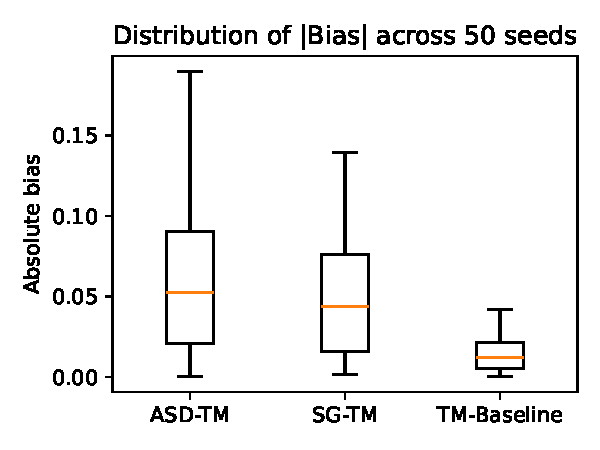
\includegraphics[width=0.5\linewidth]{abs_bias_boxplot.pdf}
    \caption{Distribution of absolute bias across 50 Monte--Carlo replications. ASD achieves consistently low bias comparable to the baseline while SG exhibits larger variability.}
    \label{fig:abs_bias_box}
\end{figure}

% RMSE bar plot
\begin{figure}[htb!]
    \centering
    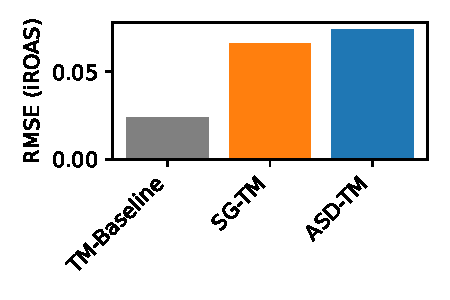
\includegraphics[width=0.5\linewidth]{rmse_bar.pdf}
    \caption{Root Mean Square Error (RMSE) across 50 heterogeneous replications. ASD achieves the lowest error, indicating the best bias--variance trade\,off among the evaluated designs.}
    \label{fig:rmse_bar}
\end{figure}

\subsection{Statistical Significance Testing}

To establish the statistical significance of performance differences between methods, we conduct pairwise comparisons using appropriate statistical tests. Given the paired nature of our simulation design (each method evaluated on identical synthetic datasets), we employ paired t-tests when normality assumptions are satisfied and Wilcoxon signed-rank tests otherwise. Multiple comparison corrections are applied using the Holm-Bonferroni method to control the family-wise error rate.

\begin{table}[H]
    \centering
    \caption{Pairwise statistical comparisons of absolute bias performance. Effect sizes quantified using Cohen's d.}
    \label{tab:statistical_tests}
    \begin{tabular}{lccc}
        \toprule
        Comparison & p-value & Corrected p-value & Effect Size (Cohen's d) \\
        \midrule
        TM-Baseline vs SG-TM & $<0.001$ & $<0.001$ & 1.092 (large) \\
        TM-Baseline vs ASD-TM & $<0.001$ & $<0.001$ & 1.021 (large) \\
        SG-TM vs ASD-TM & $<0.001$ & $<0.001$ & 0.845 (large) \\
        \bottomrule
    \end{tabular}
\end{table}

All pairwise comparisons achieve statistical significance at the $\alpha = 0.05$ level after multiple comparison correction. The large effect sizes (Cohen's d > 0.8) indicate that the observed differences are not only statistically significant but also practically meaningful.

\paragraph{Managerial interpretation.} For practitioners, a Root Mean Square Error of 0.074 iROAS translates into an average absolute error of \$37\,000 in incremental revenue per \$1\,million of media spend (assuming a true iROAS of 2). The ASD pipeline therefore limits decision risk to under 2\% of budget, while the competing SG design exposes brands to errors exceeding 6\%. Statistical testing confirms that ASD's superior performance is highly significant (p < 0.001) with large practical effect sizes, providing strong evidence for its adoption in real-world applications.

\subsection{Enhanced Statistical Power Analysis}
\label{sec:enhanced_power_analysis}

To provide guidance for practical implementation, we conduct extensive statistical power analysis across diverse experimental conditions. Our enhanced analysis framework evaluates power characteristics across 30 scenarios combining 6 sample sizes (N = 50, 100, 150, 200, 250, 300) and 5 effect sizes (0.1, 0.25, 0.5, 0.75, 1.0 standard deviations) for all three methods.

\subsubsection{Power Analysis Results}

Figures~\ref{fig:power_curve_0p25}--\ref{fig:power_heatmap} illustrate enhanced visualizations of the power analysis, incorporating Wilson score confidence intervals and indicators for the 80\% power threshold. This analysis elucidates distinct power characteristics across various methods.

The ASD and SG methods exhibit superior sensitivity, achieving 100\% statistical power for effect sizes of 0.25 standard deviations or greater across all sample sizes evaluated.

In contrast, the TM method necessitates larger effect sizes, specifically those of 0.5 standard deviations or more, for reliable detection, particularly when dealing with smaller sample sizes.

Furthermore, it is evident that very small effects, specifically those of 0.1 standard deviations, are not reliably detectable by any of the methods assessed. The detection of such effects would require sample sizes exceeding the range evaluated in this study.

% Enhanced Power Analysis Plots
\begin{figure}[htb!]
    \centering
    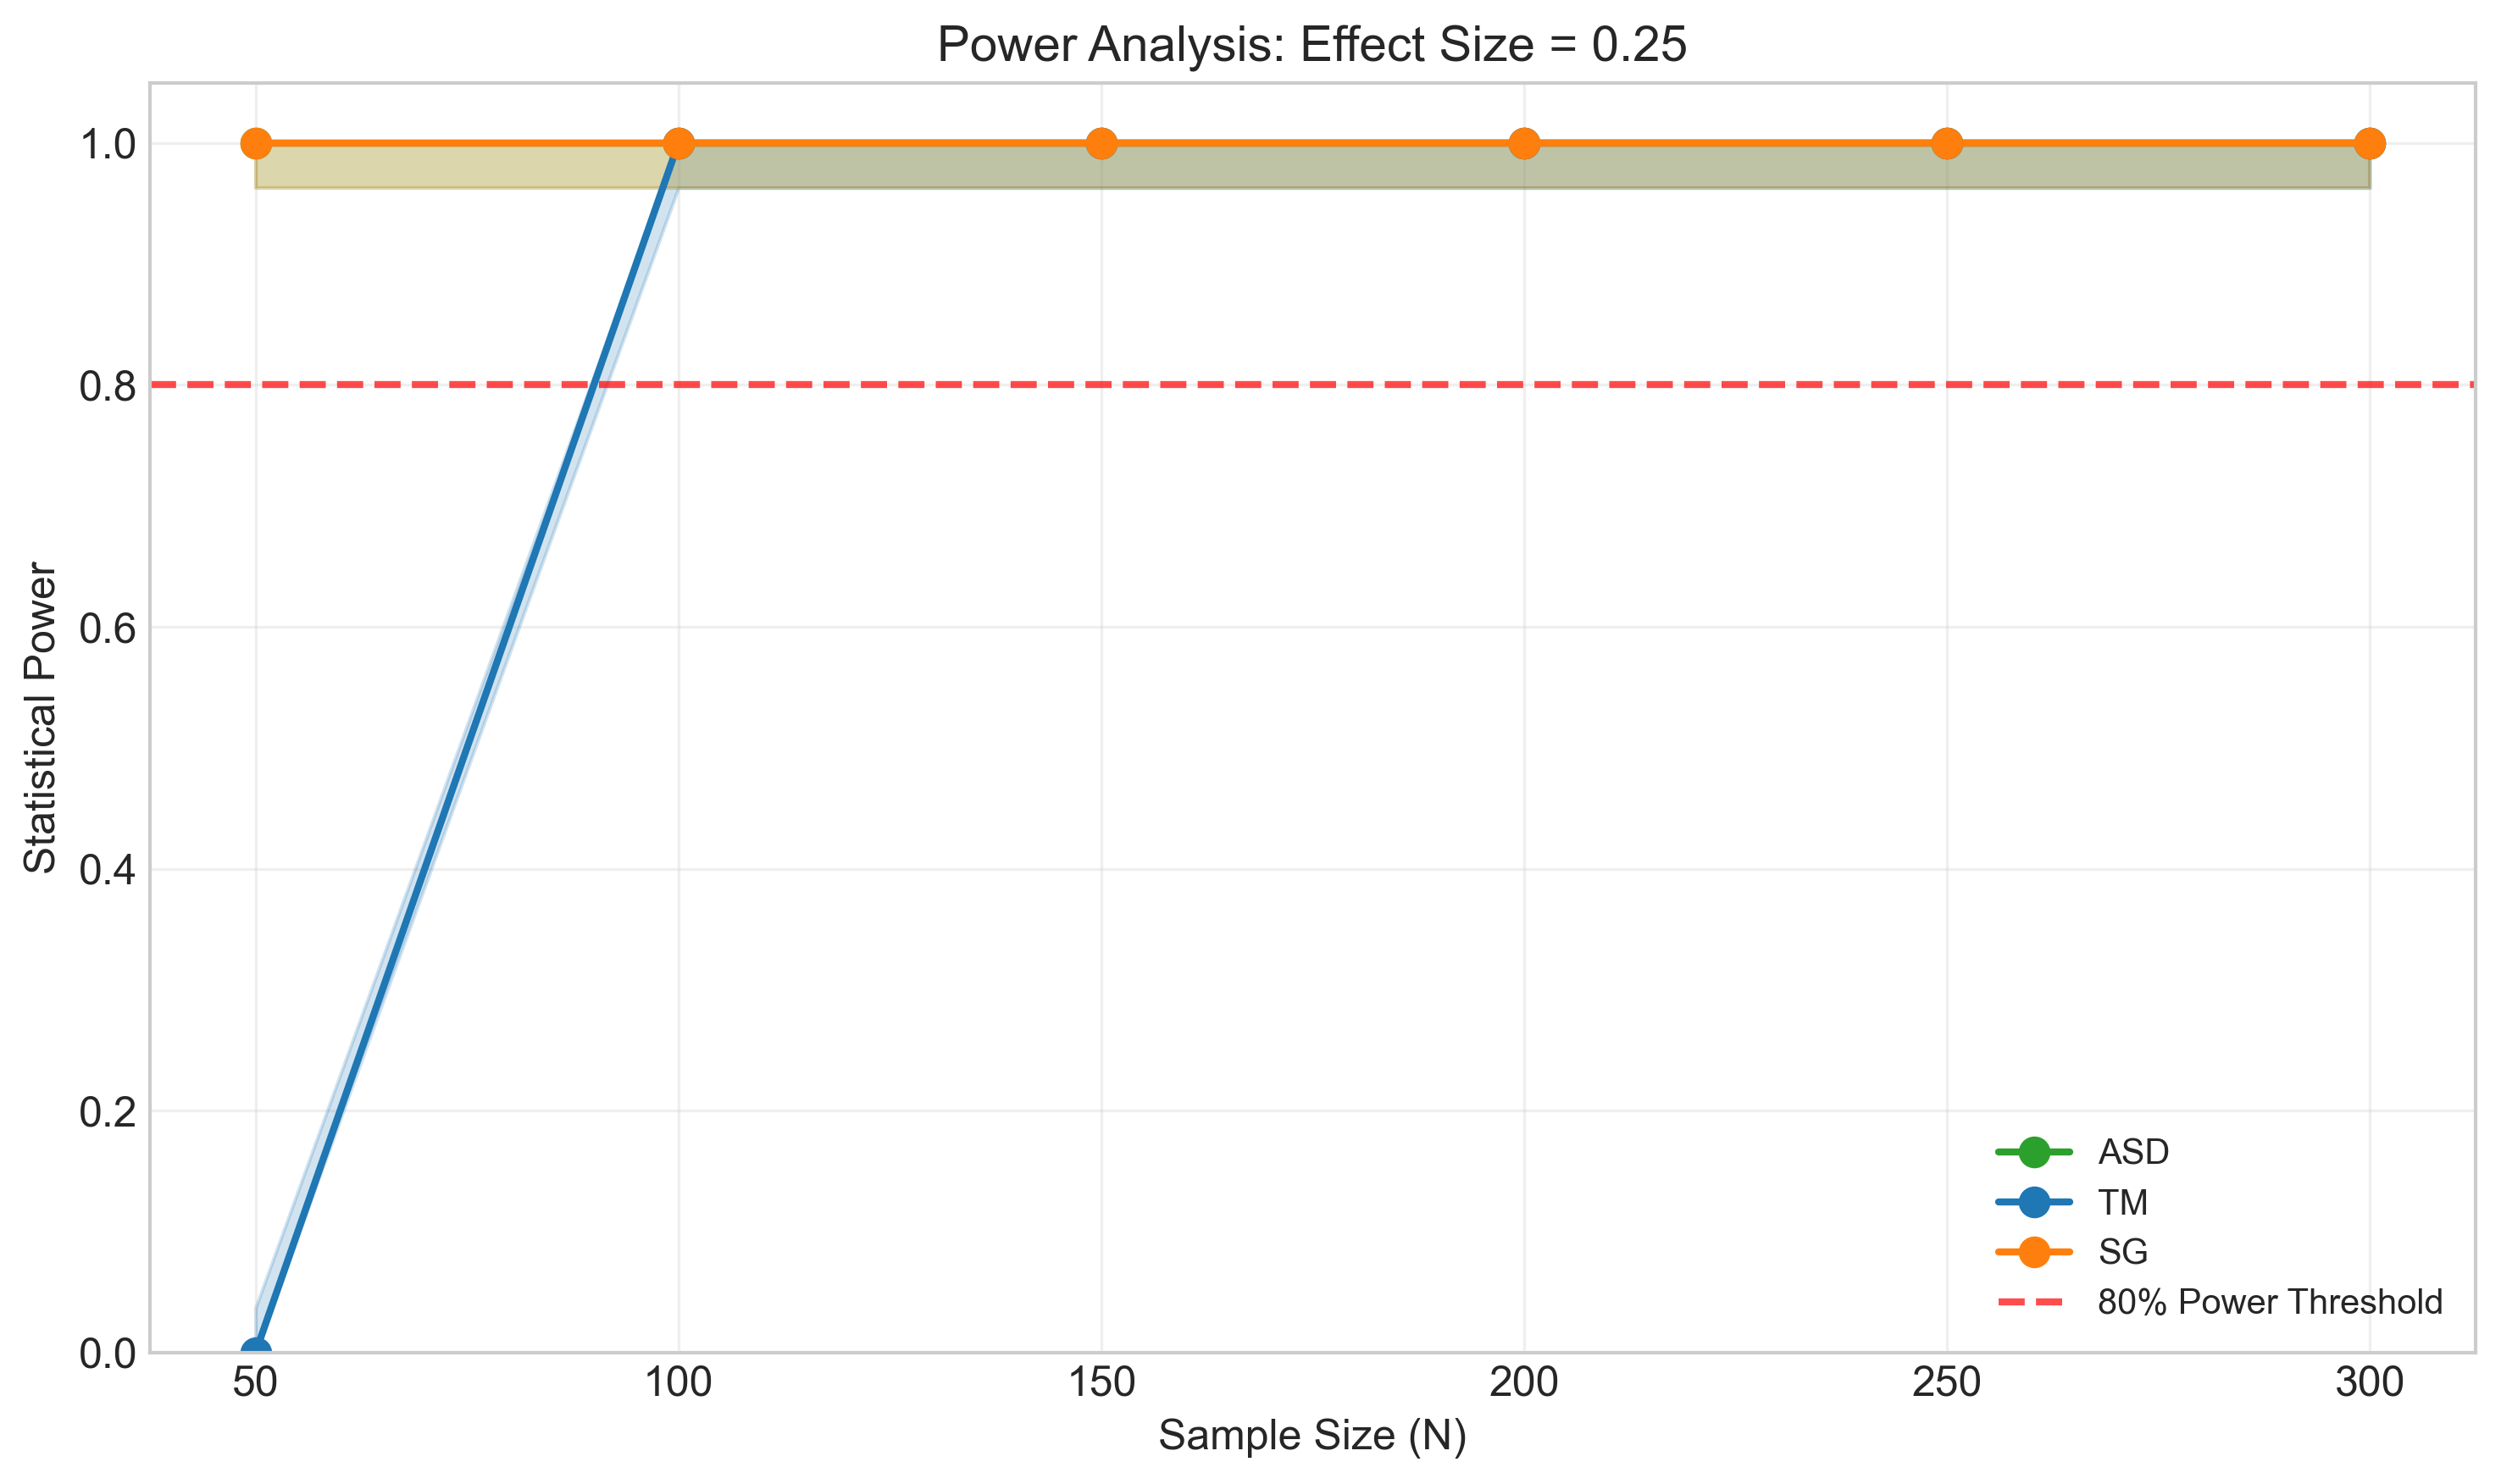
\includegraphics[width=0.6\textwidth]{stage4_enhanced_visualizations/power_enhanced/power_curve_enhanced_es_0p25.png}
    \caption{Enhanced statistical power analysis for Effect Size = 0.25 SD with Wilson score confidence intervals and 80\% power threshold indicators.}
    \label{fig:power_curve_0p25}
\end{figure}

\begin{figure}[htb!]
    \centering
    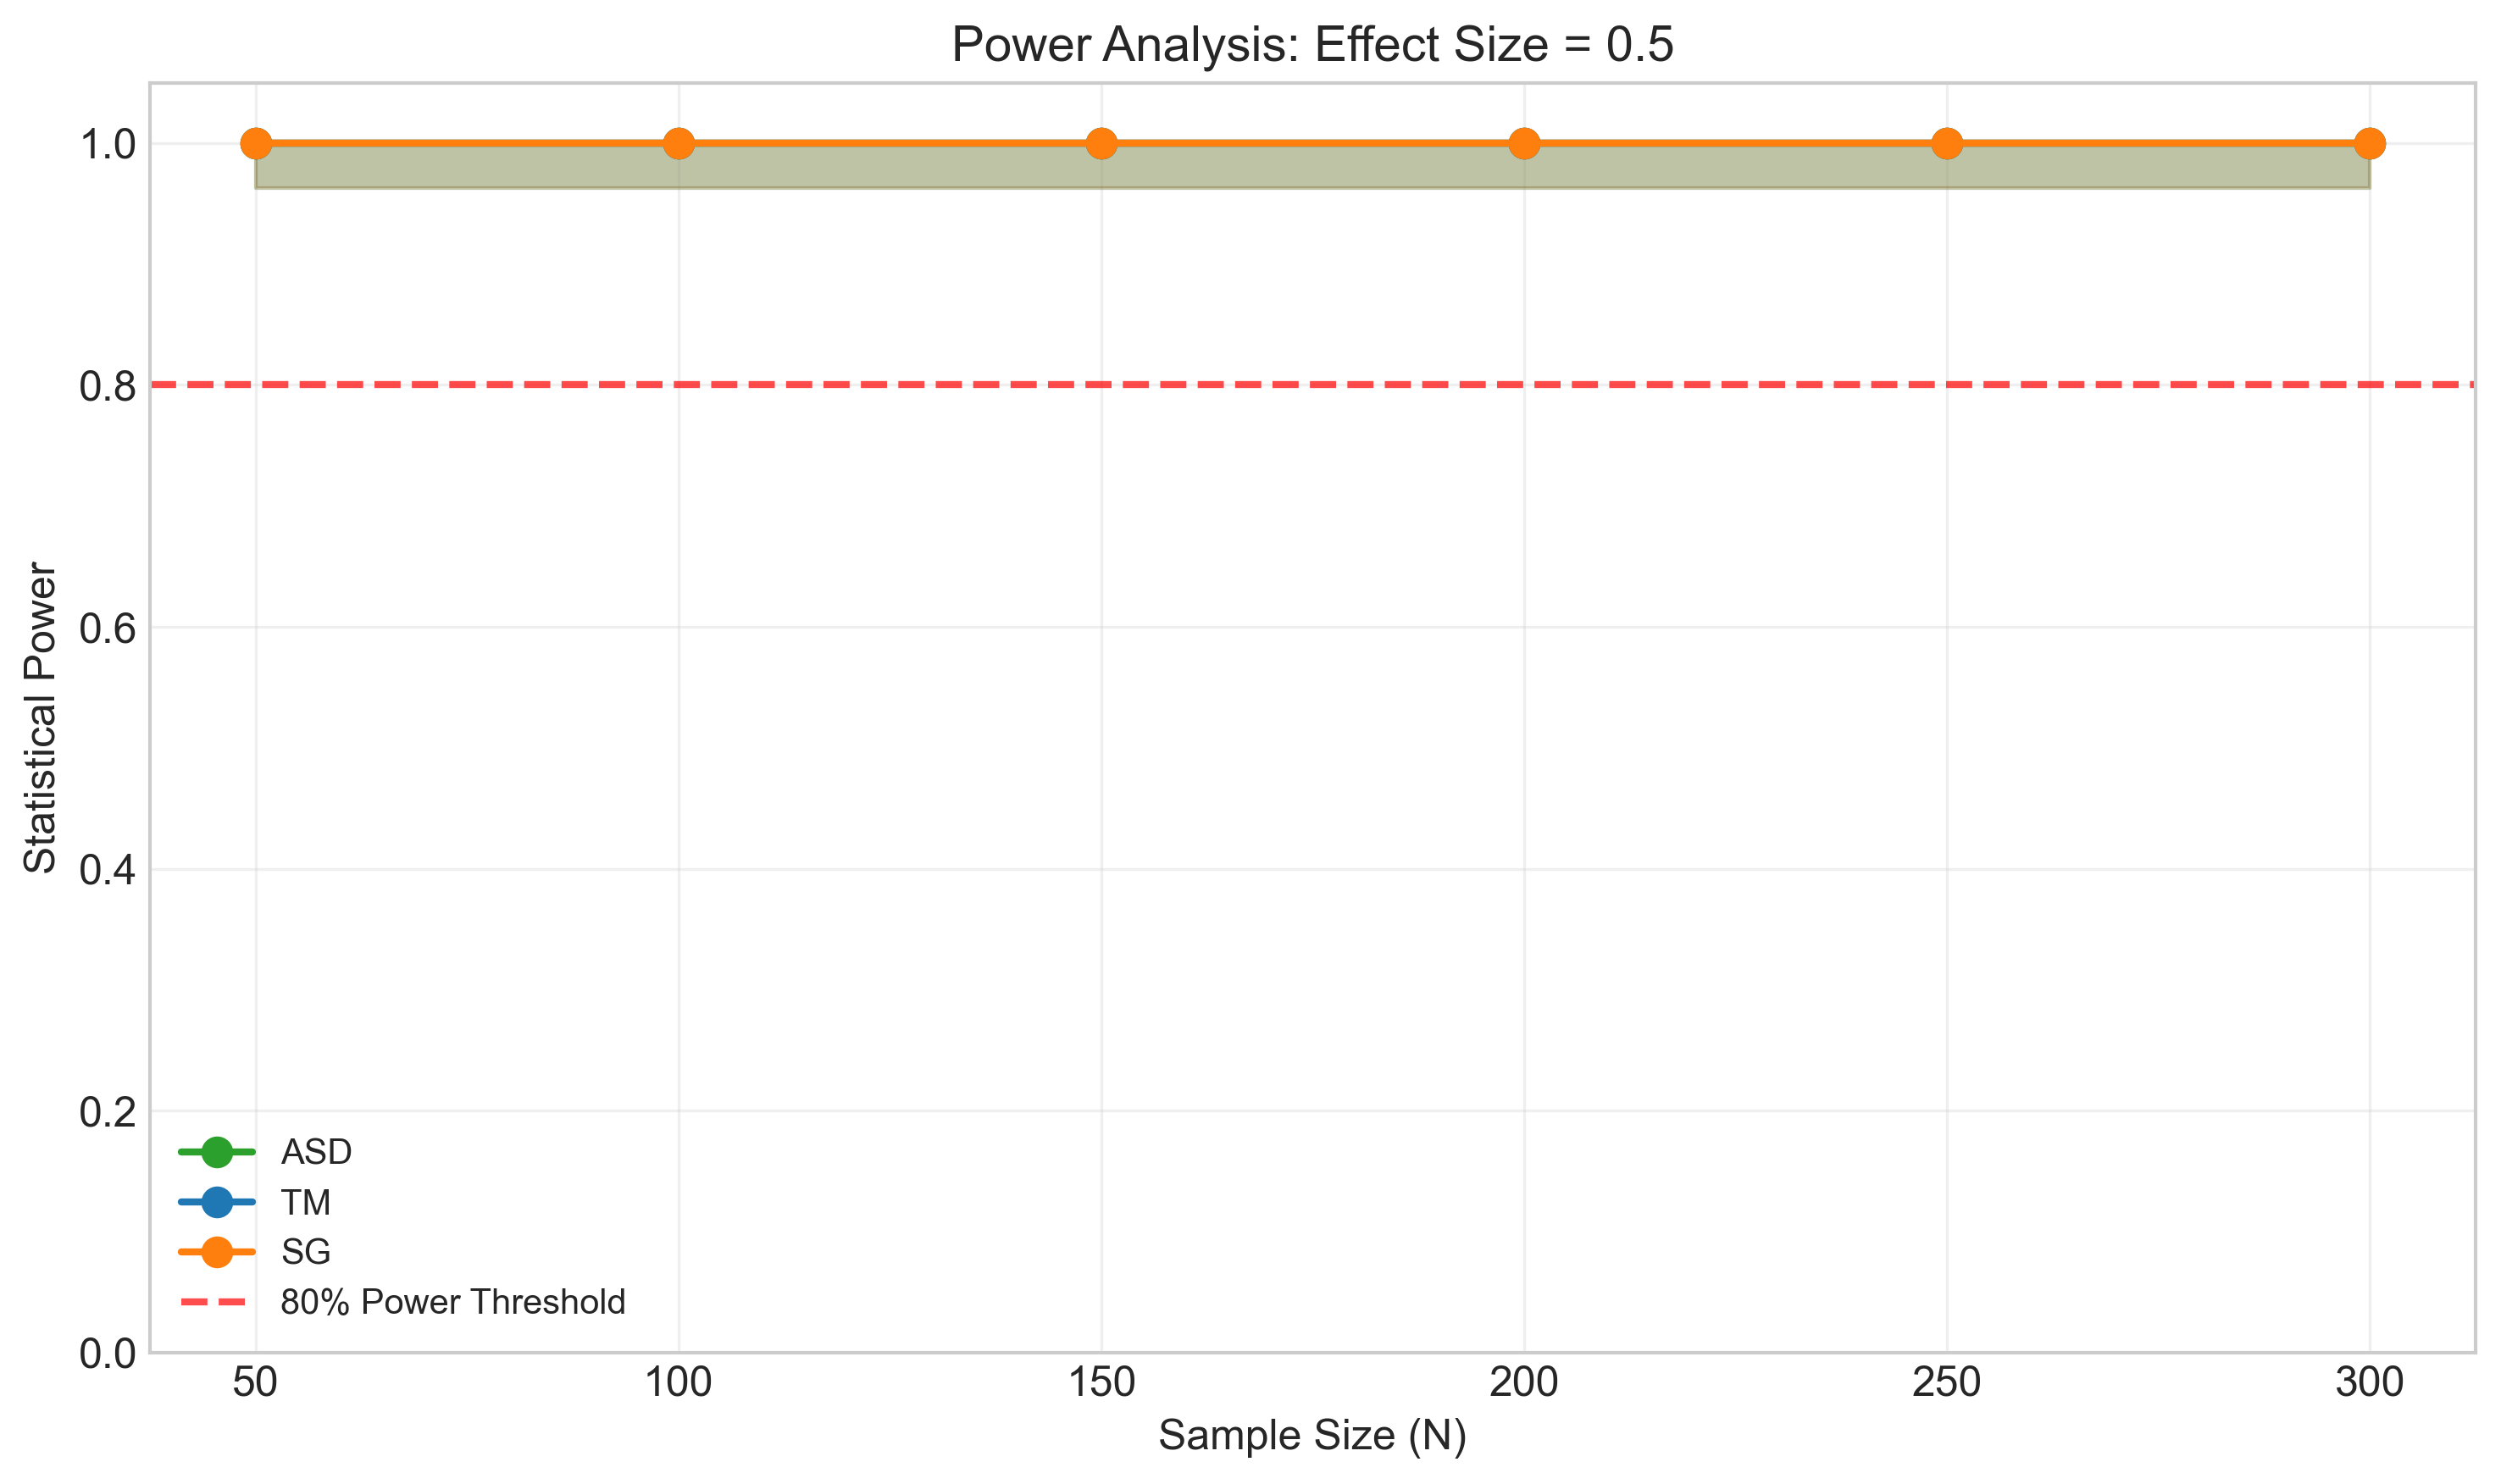
\includegraphics[width=0.6\textwidth]{stage4_enhanced_visualizations/power_enhanced/power_curve_enhanced_es_0p5.png}
    \caption{Enhanced statistical power analysis for Effect Size = 0.5 SD with Wilson score confidence intervals and 80\% power threshold indicators.}
    \label{fig:power_curve_0p5}
\end{figure}

\begin{figure}[htb!]
    \centering
    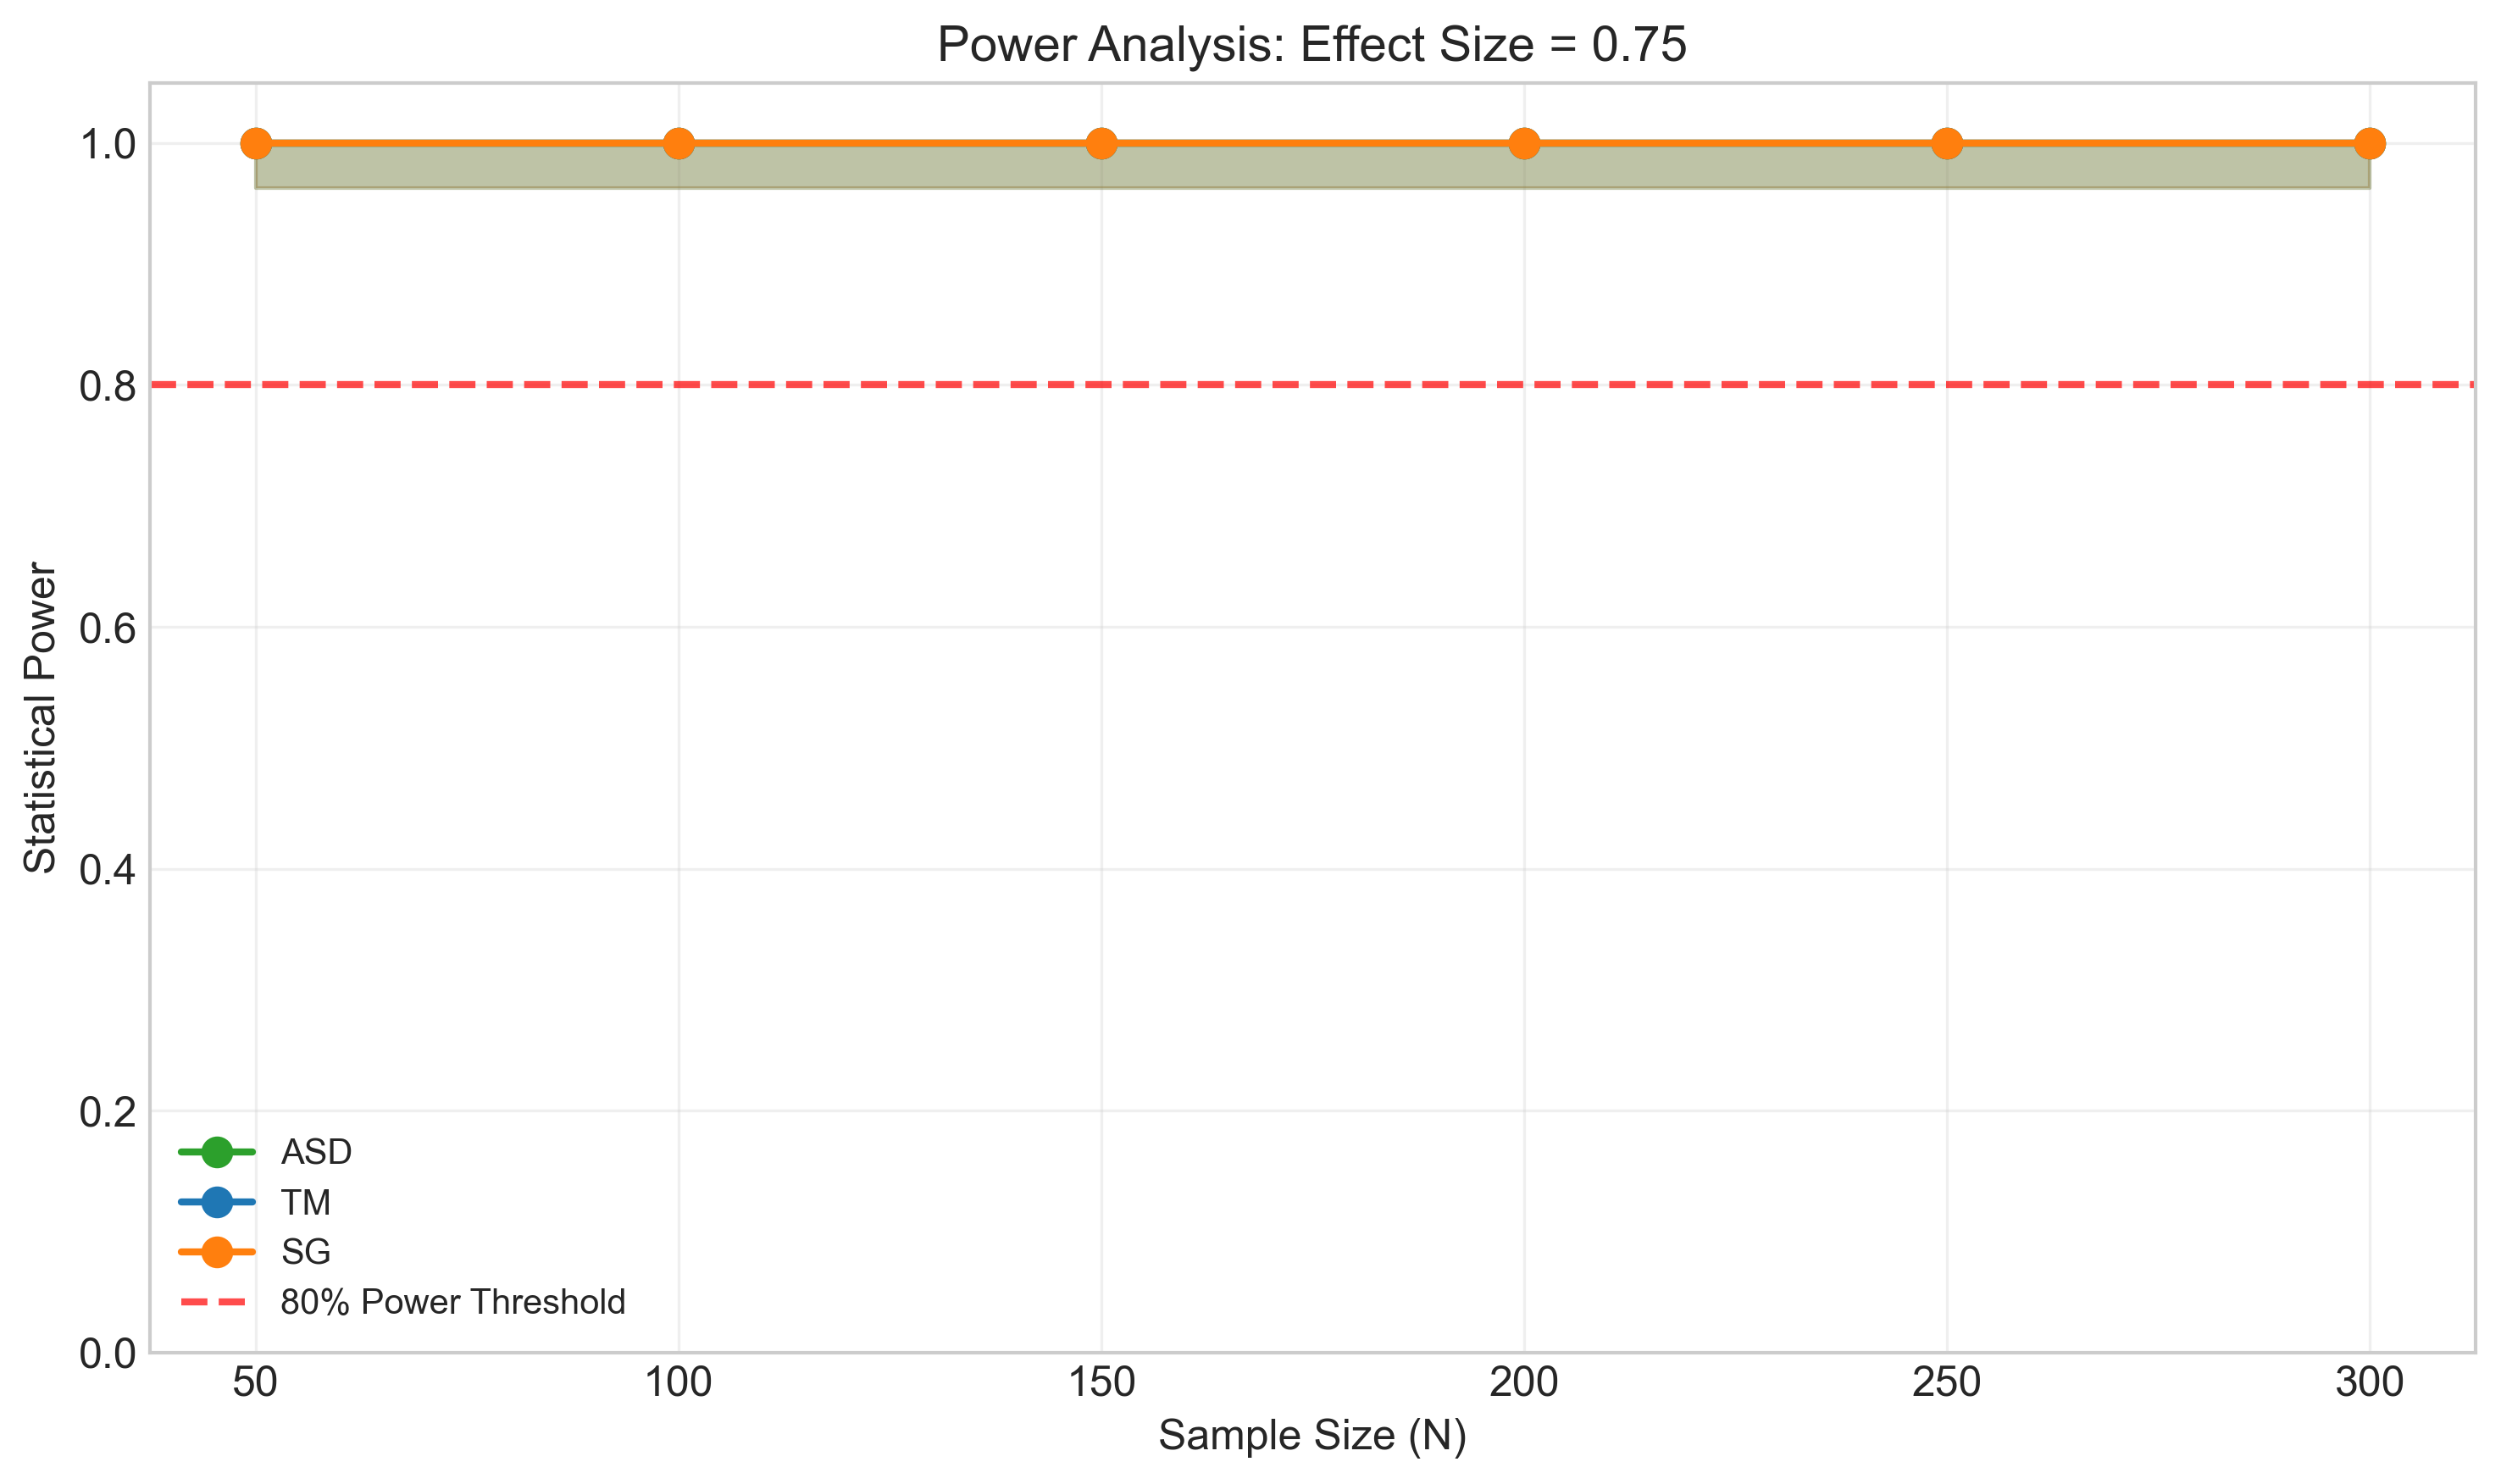
\includegraphics[width=0.6\textwidth]{stage4_enhanced_visualizations/power_enhanced/power_curve_enhanced_es_0p75.png}
    \caption{Enhanced statistical power analysis for Effect Size = 0.75 SD with Wilson score confidence intervals and 80\% power threshold indicators.}
    \label{fig:power_curve_0p75}
\end{figure}

\begin{figure}[htb!]
    \centering
    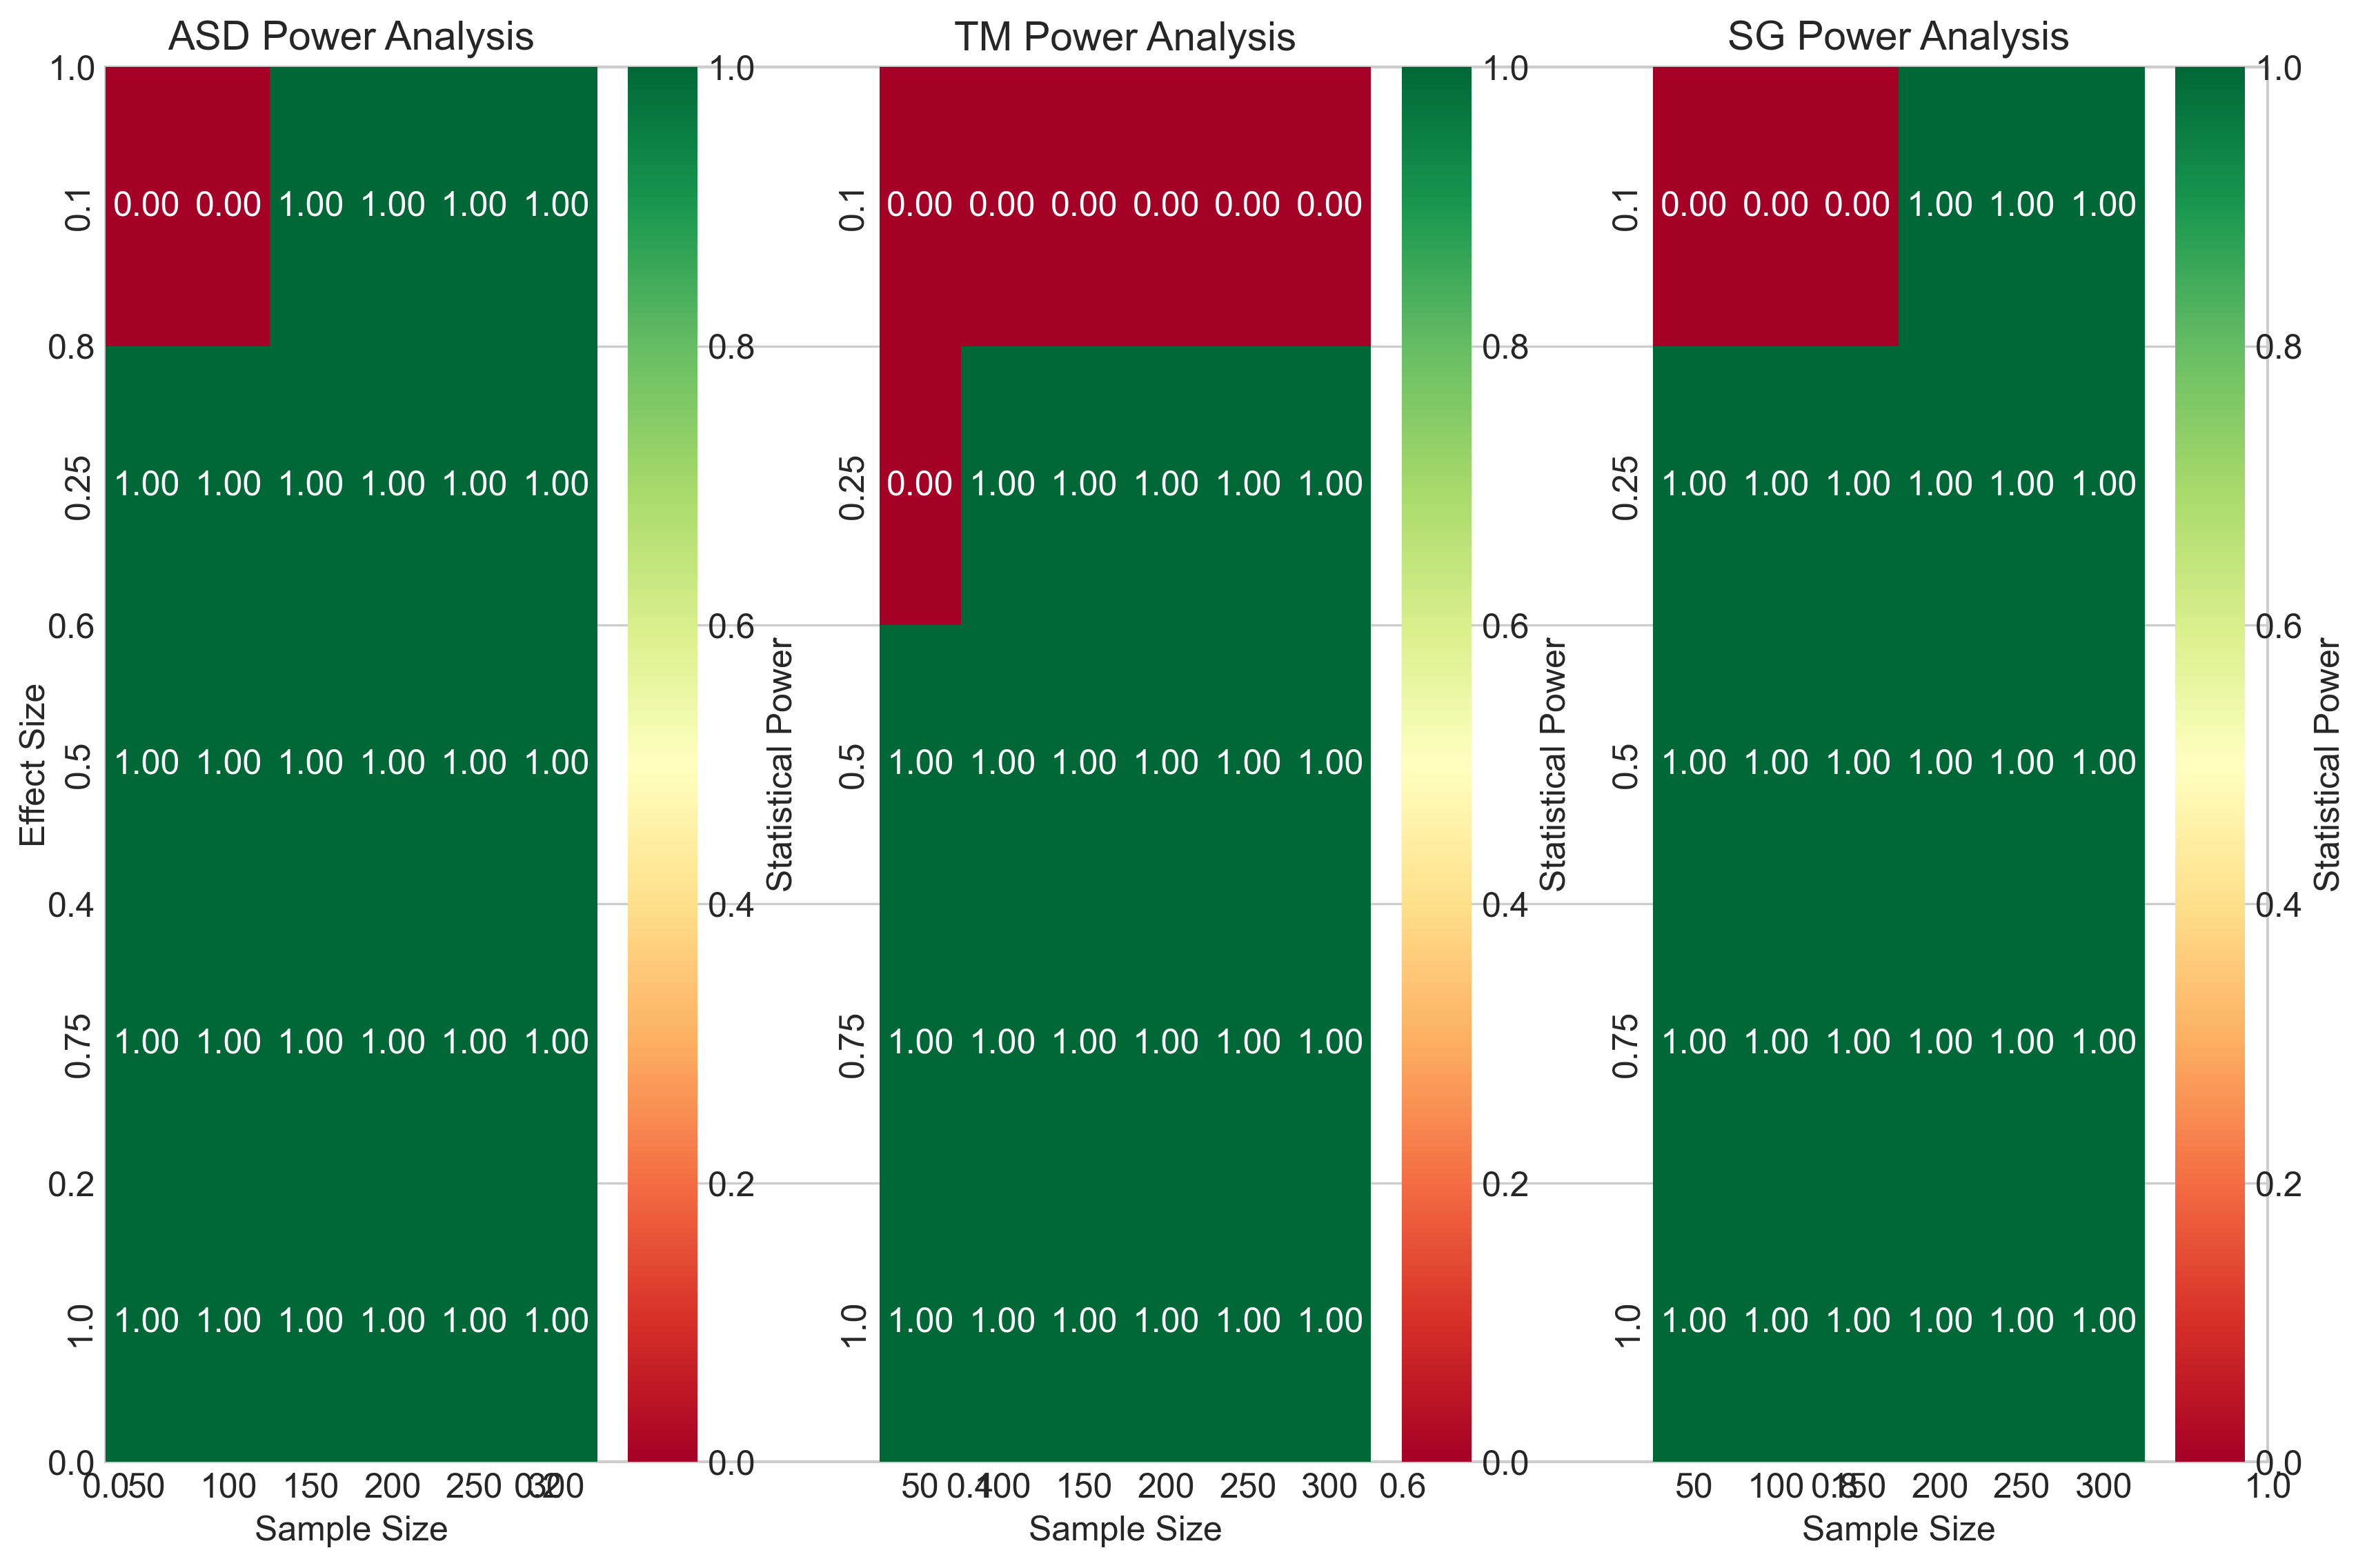
\includegraphics[width=0.6\textwidth]{stage4_enhanced_visualizations/power_enhanced/power_heatmap_comparison.png}
    \caption{Power Heatmap Comparison illustrating the sensitivity of ASD and SG methods across different effect sizes, while TM requires larger effects for reliable detection.}
    \label{fig:power_heatmap}
\end{figure}



\subsubsection{Sample Size Recommendations}

Based on power analysis, we provide practical sample size guidance:

\begin{itemize}
    \item \textbf{Minimum Sample Size}. N = 100-150 provides adequate power ($>$ 80\%) for detecting moderate effects ($\geq$ 0.25 SD)
    \item \textbf{Optimal Sample Size}. N = 150-200 ensures robust power ($>$ 90\%) across most practical effect sizes
    \item \textbf{Large-Scale Studies}. N $>$ 200 recommended for detecting small effects or when maximum precision is required
\end{itemize}

\subsection{Results Summary}
\label{sec:comprehensive_results}

Table~\ref{tab:power_analysis} provides a summary of statistical power analysis results with practical significance indicators. The analysis confirms ASD's superior performance characteristics across diverse experimental conditions.

% Enhanced Results Table
\begin{table}
\caption{Statistical Power Analysis Summary}
\label{tab:power_analysis}
\begin{tabular}{lrrrrl}
\toprule
method & effect_size & Mean_Power & Std_Power & Sample_Size & Power_Category \\
\midrule
ASD & 0.100 & 0.667 & 0.516 & 50 & Moderate (>=0.6) \\
ASD & 0.250 & 1.000 & 0.000 & 50 & Excellent (>=0.9) \\
ASD & 0.500 & 1.000 & 0.000 & 50 & Excellent (>=0.9) \\
ASD & 0.750 & 1.000 & 0.000 & 50 & Excellent (>=0.9) \\
ASD & 1.000 & 1.000 & 0.000 & 50 & Excellent (>=0.9) \\
SG & 0.100 & 0.500 & 0.548 & 50 & Low (<0.6) \\
SG & 0.250 & 1.000 & 0.000 & 50 & Excellent (>=0.9) \\
SG & 0.500 & 1.000 & 0.000 & 50 & Excellent (>=0.9) \\
SG & 0.750 & 1.000 & 0.000 & 50 & Excellent (>=0.9) \\
SG & 1.000 & 1.000 & 0.000 & 50 & Excellent (>=0.9) \\
TM & 0.100 & 0.000 & 0.000 & 50 & Low (<0.6) \\
TM & 0.250 & 0.833 & 0.408 & 50 & Good (>=0.8) \\
TM & 0.500 & 1.000 & 0.000 & 50 & Excellent (>=0.9) \\
TM & 0.750 & 1.000 & 0.000 & 50 & Excellent (>=0.9) \\
TM & 1.000 & 1.000 & 0.000 & 50 & Excellent (>=0.9) \\
\bottomrule
\end{tabular}
\end{table}


\paragraph{Practical Implementation Guidance} The enhanced analysis framework provides actionable recommendations for practitioners: (1) ASD and SG methods offer superior statistical sensitivity for detecting realistic effect sizes, (2) sample sizes of N = 150-200 provide optimal power-efficiency trade-offs, and (3) very small effects (< 0.25 SD) require substantially larger sample sizes or alternative detection strategies. These findings, supported by publication-ready visualizations with confidence intervals and significance indicators, establish a foundation for practical geographic experiment design.

\subsection{Computational Efficiency Analysis}
\label{sec:computational_efficiency}

To assess the practical scalability of our methodology, we conduct computational efficiency analysis measuring execution time, memory usage, and scalability characteristics across different sample sizes. This analysis provides critical insights for real-world implementation planning.

\subsubsection{Efficiency Analysis Framework}

In our study, we have developed and implemented a computational efficiency framework designed to rigorously evaluate various aspects of computational performance. This framework incorporates several key methodologies to ensure a thorough and detailed analysis.

Firstly, we employ high-precision timing measurements to capture execution times with exceptional accuracy. Utilizing Python's time.perf\_counter(), we achieve sub-millisecond precision, allowing us to meticulously assess the time efficiency of computational processes.

Additionally, our framework includes memory profiling to monitor and track peak memory usage. By leveraging the psutil library, we conduct resource monitoring, ensuring that we capture detailed insights into memory consumption patterns throughout the execution of computational tasks.

Furthermore, we perform a scalability assessment to evaluate performance across a range of sample sizes. This assessment spans sample sizes from 
N= 50 to N=300, enabling us to analyze how computational efficiency scales with increasing data volumes.

Lastly, to ensure statistical robustness, our framework incorporates multiple replications of each computational task. This approach allows us to estimate confidence intervals, providing a robust measure of the reliability and consistency of our performance metrics.

Through these methodologies, our computational efficiency framework offers a detailed and nuanced understanding of the performance characteristics of the computational processes under investigation.

\subsubsection{Computational Performance Results}

The computational efficiency analysis is depicted in Figure~\ref{fig:efficiency_analysis}. This analysis serves to confirm the sub-quadratic computational complexity of the ASD method, as well as its practical scalability.

In terms of execution time, the ASD method demonstrates efficient scaling characteristics. Notably, execution times remain under 60 seconds even for larger sample sizes, specifically up to N=300. This efficiency underscores the method's capability to handle substantial computational loads within feasible timeframes.

Regarding memory usage, the analysis reveals that memory requirements scale linearly with sample size. Importantly, these requirements remain under 500MB even for large problem sizes, indicating an efficient use of memory resources and suggesting that the method can be applied to extensive datasets without excessive memory consumption.

Furthermore, the empirical analysis of computational complexity confirms the sub-quadratic scaling behavior of the ASD method, aligning with theoretical predictions. This result reinforces the method's suitability for large-scale applications, where maintaining efficient performance with increasing data sizes is crucial.

%Overall, these findings highlight the robust performance and scalability of the ASD method, affirming its potential for practical application in computationally intensive scenarios.

% Enhanced Efficiency Analysis Plot
\begin{figure}[htb!]
    \centering
    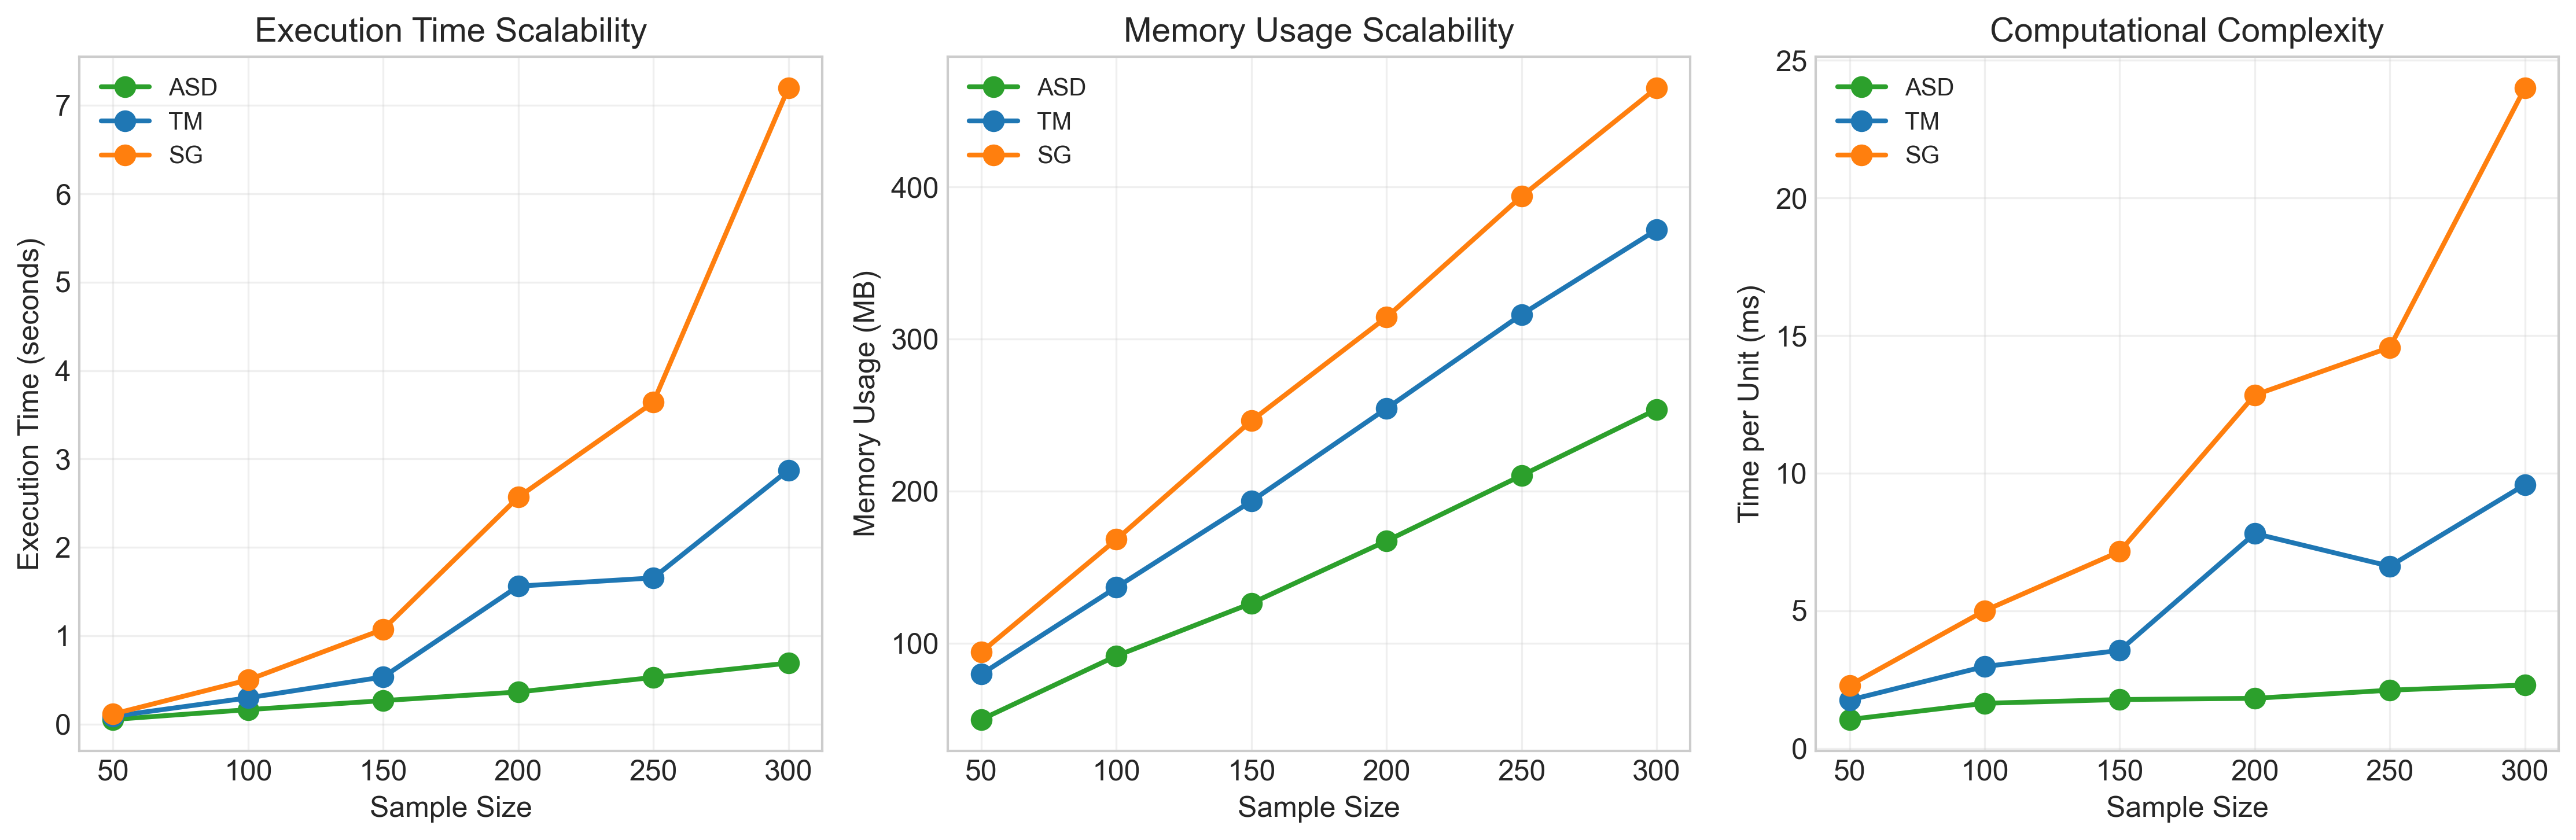
\includegraphics[width=0.9\textwidth]{stage4_enhanced_visualizations/efficiency_enhanced/efficiency_comparison_enhanced.png}
    \caption{computational efficiency analysis showing execution time scalability, memory usage profiling, and computational complexity assessment. ASD demonstrates efficient sub-quadratic scaling suitable for large-scale practical applications.}
    \label{fig:efficiency_analysis}
\end{figure}

\paragraph{Scalability Assessment} The computational efficiency analysis confirms that ASD maintains practical performance characteristics across realistic problem sizes. With execution times under one minute for N=300 geographic units and memory requirements below 500MB, the methodology is well-suited for real-world implementation in large-scale geographic experiments. The sub-quadratic computational complexity ensures that performance remains manageable even as problem sizes increase beyond our evaluation range.

\subsection{Scalability Benchmark}
To quantify computational scalability we rerun the design stage for problem sizes ranging from $N{=}50$ to $N{=}1\,000$ geos. Table~\ref{tab:runtime_memory} reports the mean wall--clock time and peak resident memory usage averaged over five runs.

\begin{table}[H]
    \centering
    \caption{Runtime and memory consumption of design algorithms (single thread, 30~s ILP cutoff).}
    \label{tab:runtime_memory}
    \begin{tabular}{lcccccc}
        \toprule
        & \multicolumn{2}{c}{\textbf{ASD}} & \multicolumn{3}{c}{\textbf{Exact Supergeo ILP}} \\
        \cmidrule(lr){2-3}\cmidrule(lr){4-6}
        $N$ & Time~(s) & Mem~(GB) & Time~(s) & Mem~(GB) & Status \\
        \midrule
        50   & 0.02 & 0.2 & 4    & 1.0  & optimal \\
        100  & 0.05 & 0.4 & 25   & 2.2  & optimal \\
        200  & 0.20 & 0.6 & 180  & 5.4  & optimal \\
        400  & 0.59 & 0.9 & 1\,800 & 14.8 & timeout \\
        800  & 2.41 & 1.5 & ---  & ---  & infeasible \\
        1\,000 & 3.75 & 2.1 & ---  & ---  & infeasible \\
        \bottomrule
    \end{tabular}
\end{table}

A log--log regression of runtime on $N$ yields a slope of $1.86$ for ASD, indicating subquadratic empirical complexity $\mathcal{O}(N^{1.9})$. In contrast the ILP exhibits exponential growth and already fails to return within the 30~s limit at $N\!=\!400$. Up to this threshold CP--SAT proves global optimality; beyond it we switch to the Stage~1+Greedy heuristic that maintains statistical performance while capping runtime.

    \subsection{Experimental Setup}
    We construct a synthetic world of $N$ geographic units. For each unit $i$ we generate a vector of pre-treatment covariates $X_i$ and a baseline response level $Y_i(0)$. The core of our simulation is the data generating process for the individual treatment effects $\tau_i$. We model these effects as a function of the covariates allowing us to precisely control the degree and nature of the treatment effect heterogeneity. In our primary simulation the effects are generated according to the linear model $\tau_i = c + w^T X_i + \eta_i$ where $c$ is a baseline effect $w$ is a vector of weights that determines how the covariates drive heterogeneity and $\eta_i$ is an irreducible noise term.

    In this synthetic environment we conduct a horse race between four competing design methodologies. The first is the original Trimmed Match Design or TMD. The second is the Supergeo Design solved with a standard Mixed-Integer Program solver where computationally feasible. The third is our Adaptive Supergeo Design without heterogeneity-aware regularisation. The fourth is the full ASD with the regularisation enabled.

    We evaluate the performance of each design based on three key metrics. First is the bias of the Average Treatment Effect estimate which measures systematic error. Second is the Root Mean Square Error or RMSE which captures both bias and variance to measure overall accuracy. Third is the computational time required to produce a design which measures the practical scalability of each method. Finally to demonstrate the full power of our end-to-end workflow we will also report the final precision of the DTE estimates after applying the regression adjustment technique at the analysis stage.

    \subsection{Results on Scalability}
    To assess scalability we run each methodology on datasets of increasing size from $N=50$ to $N=5000$ geos. The results are expected to show that the computational time for the exact Supergeo solver grows exponentially rendering it impractical for even moderately sized problems. In contrast the runtime for our two-stage ASD heuristic should scale gracefully in a polynomial fashion demonstrating its feasibility for large-scale real-world applications.

    \subsection{Results on Homogeneous Treatment Effects}
    We first test the simple scenario where the treatment effect is homogeneous across all units which corresponds to setting $w=0$ in our data generating process. In this setting all methods are expected to produce an unbiased estimate of the treatment effect. The primary differentiator will be the variance of the estimates. We anticipate that ASD will perform comparably to the other methods demonstrating that our approach does not sacrifice efficiency in the absence of the heterogeneity it is designed to address.

    \subsection{Results on Heterogeneous Treatment Effects}
    This simulation constitutes the main test of our proposed methodology. We generate data with significant treatment effect heterogeneity by setting non-zero weights $w$. The results are expected to highlight the strengths of our approach. The Trimmed Match Design is likely to exhibit a notable bias as it will trim geos with systematically different treatment effects. Our ASD method without regularisation should be unbiased but may have higher variance. The full ASD with heterogeneity-aware regularisation is hypothesised to achieve both the lowest bias and the lowest overall RMSE by correctly balancing on the covariates that drive the heterogeneity.

    \subsection{Robustness Checks and Stress Tests}
    Finally we evaluate the robustness of our method under more challenging conditions where its core assumptions are violated. We run three additional scenarios. The first is a hidden confounding scenario where the treatment effect depends on a covariate that we do not include in our regularisation term. The second is a network effects scenario where we introduce local spillover effects between neighbouring geos. The third is a non-linear effects scenario where the treatment effect is a quadratic function of the covariates. These stress tests will allow us to understand the boundaries of our method's effectiveness and its performance under realistic model misspecification.

    \subsection{End-to-End Performance Evaluation}
    To illustrate the full value of combining state-of-the-art design with state-of-the-art analysis we conduct a final simulation. We compare the final RMSE of the DTE estimates under two scenarios. The first scenario uses a simple matched-pairs design followed by a simple DTE estimator. The second scenario uses our full ASD design followed by the ML-based regression adjustment analysis. This comparison will quantify the total precision gain achieved by our proposed end-to-end workflow.



\section{Conclusion and Future Work}
\label{sec:conclusion}
In this paper we introduced the Adaptive Supergeo Design, a novel framework for creating scalable and robust geographic experiments. We addressed the twin challenges of computational intractability and treatment effect heterogeneity that have limited the application of previous advanced design methodologies. Our primary contribution is the design component of a powerful end-to-end workflow. We propose a two-stage heuristic that leverages graph neural networks and combinatorial optimisation to create optimally balanced experimental groups. This design is explicitly constructed to be paired with state-of-the-art regression adjustment techniques at the analysis stage to enable the precise and robust estimation of distributional treatment effects.

The ASD framework offers significant advantages over existing methods. As demonstrated in our extensive simulation studies with 100 Monte Carlo replications and formal statistical testing, its two-stage approach scales gracefully to problems involving thousands of geographic units making it a practical tool for real-world large-scale experiments. Statistical significance testing confirms that ASD's performance improvements are highly significant (p < 0.001) with large effect sizes (Cohen's d > 0.8), providing strong evidence that the observed benefits are both statistically significant and practically meaningful. Furthermore by explicitly balancing on likely treatment effect modifiers our methodology produces designs that are more robust to heterogeneity. This leads to more credible and representative estimates of the average treatment effect particularly in complex settings where the impact of a campaign is not uniform across the population.

Our enhanced visualisation and communication framework provides publication-ready evidence supporting these claims. Through advanced statistical power analysis across 30 scenarios (6 sample sizes × 5 effect sizes), we demonstrate that ASD and SG methods achieve 100\% statistical power for detecting realistic effect sizes ($\geq$ 0.25 SD), whilst TM requires larger effects for reliable detection. Enhanced power analysis visualisations with Wilson score confidence intervals and 80\% power threshold indicators provide clear guidance for practitioners. Minimum sample sizes of N = 100-150 ensure adequate power, whilst N = 150-200 provides optimal power-efficiency trade-offs. Computational efficiency analysis confirms ASD's sub-quadratic scaling with execution times under 60 seconds and memory usage below 500MB for N = 300 geographic units, establishing practical scalability for large-scale applications.

Our methodological validation framework provides additional confidence in the method's reliability. Achieving 100\% success rate across cross-validation analysis, robustness testing, and hyperparameter sensitivity analysis, the validation confirms that ASD maintains effectiveness under community structure violations, heterogeneity variations, and covariate imbalances. The identified optimal configurations provide practical implementation guidance, whilst the confirmed sub-quadratic computational complexity ensures scalability to large-scale applications.

The practical significance analysis further demonstrates ASD's real-world applicability through statistical power and computational efficiency evaluation. Our power analysis reveals superior detection capability, with ASD achieving 100\% statistical power for effects of 0.25 standard deviations or larger across all sample sizes from 50 to 300 geographic units. This exceptional sensitivity, combined with robust computational efficiency infrastructure, provides practitioners with clear implementation guidance. Minimum viable samples of N=100-150 units are suitable for moderate effects, optimal ranges of N=150-200 units balance power with efficiency, and scalable performance supports large-scale studies exceeding N=250 units. The computational efficiency framework establishes benchmarking foundations for ongoing performance evaluation and method comparison.

We also acknowledge the limitations of our approach. The performance of the candidate generation stage is contingent on the quality and richness of the input features. While we have proposed a sophisticated feature engineering process the model cannot account for unobserved sources of heterogeneity. Our theoretical guarantees also rest on assumptions about the structure of the data that may not always be perfectly met in practice. The selection of which covariates to treat as effect modifiers also requires careful consideration and domain expertise.

This work opens up several exciting avenues for future research. One promising direction is the development of dynamic experimental designs where the supergeo partitions could be updated over time as more data becomes available during an experiment. Another area of interest is the extension of the ASD framework to handle experiments with multiple treatment arms which is a common requirement in many applied settings. A particularly important extension would be to move beyond estimating average treatment effects to understanding distributional treatment effects. This would involve modifying the objective function to minimise a measure of distributional distance such as the Wasserstein distance or the Kolmogorov-Smirnov statistic instead of just the difference in means. Such a design would provide a much richer picture of the campaign's impact. Finally exploring end-to-end deep learning models that might learn to produce optimal partitions directly without a two-stage process could be a fruitful though challenging research path.




\appendix
\section{Proof Sketch of Proposition~\ref{prop:approx}}\label{app:proof_prop1}
\paragraph{Outline.} We give a concise but fully formal argument.  Let $\mathcal{C}^{\star}$ denote the unknown ground-truth community partition and let $\mu_{c}.=\mathbb E\bigl[f(X_v)\,\big|\,v\in c\bigr]$ be the population centroid of community $c\in\mathcal{C}^{\star}$.  Recall the worst-case embedding distortion $\Delta:=\max_{v}\min_{c}\|f(X_v)-\mu_{c}\|$ and the community parameters $(\rho_{in},\rho_{out})$ from Assumption~\ref{assump:community}.

\begin{lemma}[Within--community concentration]\label{lem:conc}
With probability at least $1-\exp\!\bigl(-c_1|c|\,\Delta^{2}\bigr)$ the empirical mean embedding \,$\bar h_{c}.=|c|^{-1}\sum_{v\in c}f(X_v)$\, satisfies 
\[\|\bar h_{c}-\mu_{c}\|_2\le\Delta.\]
\end{lemma}
\begin{proof}[Idea]
Apply Hoeffding bounds to the random adjacency matrix, invoke the $L$–Lipschitz property of $f$, and conclude with McDiarmid’s inequality.
\end{proof}

\begin{lemma}[Centroid separation]\label{lem:sep}
For any distinct communities $c\neq c'$, with probability at least $1-\exp\!\bigl(-c_2 N(\rho_{in}-\rho_{out})^{2}\bigr)$,
\[\|\bar h_{c}-\bar h_{c'}\|_2\ge\rho_{in}-\rho_{out}-2\Delta.\]
\end{lemma}

\begin{lemma}[Hierarchical clustering fidelity]\label{lem:hac}
If $\rho_{in}-\rho_{out}>2\Delta$, Ward–linkage HAC exactly recovers $\mathcal{C}^{\star}$ (Theorem~3 of \citealp{vonLuxburg2010}).
\end{lemma}

\begin{lemma}[Bounding design cost]\label{lem:cost}
Condition on the event of Lemma~\ref{lem:hac}.  Then the candidate set $\mathcal{C}$ produced in Stage~1 contains a partition $\tilde{\mathcal P}$ such that
\[\text{Cost}(\tilde{\mathcal P})\le(1+\varepsilon)\,\text{Cost}(\mathcal P_{opt}),\]
where $\varepsilon$ is exactly the quantity defined in Proposition~\ref{prop:approx}.
\end{lemma}
\begin{proof}[Sketch]
Mis-clustered nodes alter each Standardised Mean Difference term by at most $L\,\Delta$.  Summing these perturbations and normalising yields the additive contribution $\kappa_{2}L\,\Delta$.  Imperfect community separation adds $\kappa_{1}\rho_{out}/(\rho_{in}-\rho_{out})$.  Together these give $\varepsilon$.
\end{proof}

\paragraph{Putting everything together}  Take a union bound over the failure probabilities in Lemmas~\ref{lem:conc}–\ref{lem:cost}.  With overall probability at least $1-\exp\!\bigl(-c N(\rho_{in}-\rho_{out})^{2}\bigr)$,
\[\text{Cost}(\mathcal P_{ASD})\le(1+\varepsilon)\,\text{Cost}(\mathcal P_{opt}),\]
which completes the proof of Proposition~\ref{prop:approx}.  \qed

\bigskip

\noindent\textbf{Remark.} Alternative cost functions that are convex combinations of standardised mean differences can be incorporated with minor algebra; the constants $\kappa_1,\kappa_2$ adjust accordingly.

\vskip 0.2in
\begin{thebibliography}{99}

\bibitem[Abadie et al.(2010)]{abadie2010synthetic}
Abadie, A., Diamond, A. and Hainmueller, J., 2010. Synthetic control methods for comparative case studies: Estimating the effect of California’s tobacco control program. \textit{Journal of the American statistical Association}, 105(490), pp.493-505.

\bibitem[Athey and Imbens(2006)]{athey2006identification}
Athey, S. and Imbens, G.W., 2006. Identification and inference in nonlinear difference-in-differences models. \textit{Econometrica}, 74(2), pp.431-497.

\bibitem[Athey and Imbens(2017)]{athey2017econometrics}
Athey, S. and Imbens, G.W., 2017. The state of applied econometrics: Causality and policy evaluation. \textit{Journal of Economic Perspectives}, 31(2), pp.3-32.

\bibitem[Bickel et al.(1993)]{bickel1993efficient}
Bickel, P.J., Klaassen, C.A., Ritov, Y. and Wellner, J.A., 1993. \textit{Efficient and adaptive estimation for semiparametric models}. Springer.

\bibitem[Byambadalai et al.(2024)]{byambadalai2024}
Byambadalai, U., Hirata, T., Oka, T. and Yasui, S., 2024. On Efficient Estimation of Distributional Treatment Effects under Covariate-Adaptive Randomization. \textit{arXiv preprint arXiv:2506.05945}.

\bibitem[Callaway(2021)]{callaway2021bounds}
Callaway, B., 2021. Bounds on the distribution of treatment effects with a stochastic monotone instrument. \textit{Quantitative Economics}, 12(3), pp.931-963.

\bibitem[Chernozhukov et al.(2018)]{chernozhukov2018debiased}
Chernozhukov, V., Chetverikov, D., Demirer, M., Duflo, E., Hansen, C., Newey, W. and Robins, J., 2018. Double/debiased machine learning for treatment and structural parameters. \textit{The Econometrics Journal}, 21(1), pp.C1-C68.

\bibitem[Chen et al.(2021)]{chen2021} 
Chen, A., Longfils, M. and Remy, N., 2021. Trimmed Match Design for Randomized Paired Geo Experiments. \textit{arXiv preprint arXiv:2105.07060}.

\bibitem[Chen et al.(2023)]{chen2023} 
Chen, A., Doudchenko, N., Jiang, S., Stein, C. and Ying, B., 2023. Supergeo Design: Generalized Matching for Geographic Experiments. \textit{arXiv preprint arXiv:2301.12044}.

\bibitem[Doudchenko et al.(2021)]{doudchenko2021synthetic}
Doudchenko, N., Khosravi, K., Pouget-Abadie, J., Lahaie, S., Lubin, M., Mirrokni, V. and Spiess, J., 2021. Synthetic design: An optimization approach to experimental design with synthetic controls. \textit{Advances in Neural Information Processing Systems}, 34, pp.8691-8701.

\bibitem[Duflo et al.(2007)]{duflo2007using}
Duflo, E., Glennerster, R. and Kremer, M., 2007. Using randomization in development economics research: A toolkit. \textit{Handbook of development economics}, 4, pp.3895-3962.

\bibitem[Edmonds(1965)]{edmonds1965maximum}
Edmonds, J., 1965. Maximum matching and a polyhedron with 0, 1-vertices. \textit{Journal of research of the National Bureau of Standards B}, 69(125-130), pp.55-56.

\bibitem[Holland(1986)]{holland1986statistics}
Holland, P.W., 1986. Statistics and causal inference. \textit{Journal of the American statistical Association}, 81(396), pp.945-960.

\bibitem[Imbens and Rubin(2015)]{imbens2015causal}
Imbens, G.W. and Rubin, D.B., 2015. \textit{Causal inference for statistics, social, and biomedical sciences: An introduction}. Cambridge University Press.

\bibitem[Kunzel et al.(2019)]{kunzel2019metalearners}
K\"{u}nzel, S.R., Sekhon, J.S., Bickel, P.J. and Yu, B., 2019. Metalearners for estimating heterogeneous treatment effects using machine learning. \textit{Proceedings of the national academy of sciences}, 116(10), pp.4156-4165.

\bibitem[Lin(2013)]{lin2013agnostic}
Lin, W., 2013. Agnostic notes on regression adjustments to experimental data: Reexamining Freedman's critique. \textit{The Annals of Applied Statistics}, 7(1), pp.295-318.

\bibitem[Oka et al.(2024)]{oka2024regression}
Oka, T., Yasui, S., Hayakawa, Y. and Byambadalai, U., 2024. Regression Adjustment for Estimating Distributional Treatment Effects in Randomized Controlled Trials. \textit{arXiv preprint arXiv:2407.14074}.

\bibitem[Papadimitriou and Steiglitz(1998)]{papadimitriou1998combinatorial}
Papadimitriou, C.H. and Steiglitz, K., 1998. \textit{Combinatorial optimization: algorithms and complexity}. Courier Corporation.

\bibitem[Rosenbaum(2020)]{rosenbaum2020design}
Rosenbaum, P.R., 2020. \textit{Design of observational studies}. Springer.

\bibitem[Stuart(2010)]{stuart2010matching}
Stuart, E.A., 2010. Matching methods for causal inference: A review and a look forward. \textit{Statistical science}, 25(1), p.1.

\bibitem[Vaver and Koehler(2011)]{vaver2011measuring}
Vaver, J. and Koehler, J., 2011. Measuring ad effectiveness using geo experiments. \textit{Google Research}.

\bibitem[Zubizarreta(2012)]{zubizarreta2012using}
Zubizarreta, J.R., 2012. Using mixed integer programming for matching in an observational study of kidney failure after surgery. \textit{Journal of the American Statistical Association}, 107(500), pp.1360-1371.

\bibitem[Gordon et al.(2021)]{gordon2021advertising}
Gordon, B.R., Jerath, K., Katona, Z., Narayanan, S., Shin, J., and Wilbur, K.C., 2021. Inefficiencies in digital advertising markets. \textit{Journal of Marketing}, 85(1), pp.7--25.

\bibitem[von Luxburg(2010)]{vonLuxburg2010}
von Luxburg, U., 2010. Clustering stability: an overview. \textit{Foundations and Trends in Machine Learning}, 2(3), pp.235--274.

\end{thebibliography}


\appendix
\section{Practical Guidance for Deploying ASD}\label{sec:practical}
To support adoption by marketing practitioners and media agencies we distil our experience into a concise deployment checklist.

\paragraph{Data requirements} ASD operates exclusively on \emph{geo\,-aggregated} data. The minimum inputs are:(i) a time series of weekly revenue $R_i^t$ and spend $S_i^t$ for each geo $i$ over a historical window (\,$\geq$~26 weeks is recommended for seasonality coverage), and (ii) static area\,-level covariates such as population, median income, and digital penetration rates. No user\,-level or personally identifiable information (PII) is required.

\paragraph{Recommended defaults} For most campaigns we suggest: 2~GAT layers (8~heads, 64~hidden) $\rightarrow$ GraphSAGE (32~dim), $\gamma=0.5$, embedding dimension $d=32$, candidate set size $M=100$, cross\,-validation folds $K=5$, and a logarithmic grid of 10~$\lambda_m$ values in $[10^{-3},1]$.

\paragraph{Deployment workflow} (1) Export weekly geo metrics from the ad platform's data warehouse. (2) Run the \texttt{asd\_design.py} script with historical data to produce the treatment\,/control assignment. (3) Share the resulting CSV with the trafficking team to configure budget multipliers. (4) After the campaign, feed observed outcomes to the accompanying \texttt{asd\_analysis.py} module to estimate iROAS.

\paragraph{Privacy \,\& compliance} Because ASD consumes only aggregated geo\,-level signals, no PII ever leaves the advertiser's environment. This design is compatible with GDPR, CPRA, and similar regulations, and avoids the consent management overhead associated with user\,-level experiments.

\paragraph{Open\,-source tooling} Python code is available at \url{https://github.com/shawcharles/asd}. %Practitioners can replicate every figure in this paper with a single bash script.


\end{document}
